% -*- Mode:TeX -*-

%% The documentclass options along with the pagestyle can be used to generate
%% a technical report, a draft copy, or a regular thesis.  You may need to
%% re-specify the pagestyle after you \include  cover.tex.  For more
%% information, see the first few lines of mitthesis.cls. 

%\documentclass[12pt,vi,twoside]{mitthesis}
%%
%%  If you want your thesis copyright to you instead of MIT, use the
%%  ``vi'' option, as above.
%%
%\documentclass[12pt,twoside,leftblank]{mitthesis}
%%
%% If you want blank pages before new chapters to be labelled ``This
%% Page Intentionally Left Blank'', use the ``leftblank'' option, as
%% above. 

\documentclass[12pt,twoside]{mitthesis}
\usepackage{lgrind}
\pagestyle{plain}

\usepackage{listings}
\lstset{numbers=left, frame=lines, tabsize=4, captionpos=b, numberstyle=\tiny}
\usepackage{url}
\usepackage{graphicx}
\usepackage{amsmath}

%% This bit allows you to either specify only the files which you wish to
%% process, or `all' to process all files which you \include.
%% Krishna Sethuraman (1990).

%\typein [\files]{Enter file names to process, (chap1,chap2 ...), or `all' to
%process all files:}
\def\files{all}
\def\all{all}
\ifx\files\all \typeout{Including all files.} \else \typeout{Including only \files.} \includeonly{\files} \fi

\usepackage{amsthm}

\theoremstyle{plain}
\newtheorem{theorem}{Theorem}
\newtheorem*{theorem*}{Theorem}
\newtheorem{lemma}{Lemma}
\newtheorem*{lemma*}{Lemma}
\theoremstyle{definition}
\newtheorem{definition}{Definition}
\newtheorem*{definition*}{Definition}


\begin{document}

% -*-latex-*-
% $Log: cover.tex,v $
% Revision 1.7  2001/02/08 18:53:16  boojum
% changed some \newpages to \cleardoublepages
%
% Revision 1.6  1999/10/21 14:49:31  boojum
% changed comment referring to documentstyle
%
% Revision 1.5  1999/10/21 14:39:04  boojum
% *** empty log message ***
%
% Revision 1.4  1997/04/18  17:54:10  othomas
% added page numbers on abstract and cover, and made 1 abstract
% page the default rather than 2.  (anne hunter tells me this
% is the new institute standard.)
%
% Revision 1.4  1997/04/18  17:54:10  othomas
% added page numbers on abstract and cover, and made 1 abstract
% page the default rather than 2.  (anne hunter tells me this
% is the new institute standard.)
%
% Revision 1.3  93/05/17  17:06:29  starflt
% Added acknowledgements section (suggested by tompalka)
% 
% Revision 1.2  92/04/22  13:13:13  epeisach
% Fixes for 1991 course 6 requirements
% Phrase "and to grant others the right to do so" has been added to 
% permission clause
% Second copy of abstract is not counted as separate pages so numbering works
% out
% 
% Revision 1.1  92/04/22  13:08:20  epeisach
\title{A Commodity Trusted Computing Module}

\author{Victor Marius Costan}
\department{Department of Electrical Engineering and Computer Science}
% If the thesis is for two degrees simultaneously, list them both
% separated by \and like this:
% \degree{Doctor of Philosophy \and Master of Science}
\degree{Master of Engineering in Computer Science and Engineering}
\degreemonth{May}
\degreeyear{2008}
\thesisdate{May 23, 2008}

%% By default, the thesis will be copyrighted to MIT.  If you need to copyright
%% the thesis to yourself, just specify the `vi' documentclass option.  If for
%% some reason you want to exactly specify the copyright notice text, you can
%% use the \copyrightnoticetext command.  
%\copyrightnoticetext{\copyright IBM, 1990.  Do not open till Xmas.}

\supervisor{Srinivas Devadas}{Associate Department Head, Professor}{Thesis
Supervisor}

\supervisor{Luis F. G. Sarmenta}{Research Scientist}{Thesis Co-supervisor}

% This is the department committee chairman, not the thesis committee
% chairman.  You should replace this with your Department's Committee
% Chairman.
\chairman{Arthur C. Smith}{Professor of Electrical Engineering}{Chairman,
Department Committee on Graduate Students}

% Make the titlepage based on the above information.  If you need
% something special and can't use the standard form, you can specify
% the exact text of the titlepage yourself.  Put it in a titlepage
% environment and leave blank lines where you want vertical space.
% The spaces will be adjusted to fill the entire page.  The dotted
% lines for the signatures are made with the \signature command.
\maketitle

% The abstractpage environment sets up everything on the page except
% the text itself.  The title and other header material are put at the
% top of the page, and the supervisors are listed at the bottom.  A
% new page is begun both before and after.  Of course, an abstract may
% be more than one page itself.  If you need more control over the
% format of the page, you can use the abstract environment, which puts
% the word "Abstract" at the beginning and single spaces its text.

%% You can either \input (*not* \include) your abstract file, or you can put
%% the text of the abstract directly between the \begin{abstractpage} and
%% \end{abstractpage} commands.

% First copy: start a new page, and save the page number.
\cleardoublepage
% Uncomment the next line if you do NOT want a page number on your
% abstract and acknowledgments pages.
% \pagestyle{empty}
\setcounter{savepage}{\thepage}
\begin{abstractpage}
% $Log: abstract.tex,v $
% Revision 1.1  93/05/14  14:56:25  starflt
% Initial revision
% 
% Revision 1.1  90/05/04  10:41:01  lwvanels
% Initial revision
% 
%
%% The text of your abstract and nothing else (other than comments) goes here.
%% It will be single-spaced and the rest of the text that is supposed to go on
%% the abstract page will be generated by the abstractpage environment.  This
%% file should be \input (not \include 'd) from cover.tex.
The Trusted Execution Module (TEM) is a high-level specification for a
commodity chip that can execute user-supplied procedures in a trusted
environment. The TEM draws inspiration from the Trusted Platform Module (TPM),
the first security-related hardware that has gained massive adoption in the PC
market. However, the TEM is capable of securely executing procedures expressing
arbitrary computation, originating from a potentially untrusted party, whereas
the TPM is limited to a set of cryptographic functions that is fixed at
design-time. Despite its greater flexibility, the TEM design was implemented on
the same inexpensive off-the-shelf hardware as the TPM, and it does not require
any export-restricted technology. Furthermore, the TEM removes the expensive
requirement of a secure binding to it  host computer. This makes TEM a great
candidate for the next-generation TPM. However, the TEM's guarantees of
secure execution enable exciting applications that were far beyond the reach of
TPM-powered systems. The applications include but are not limited to mobile
agents, peer-to-peer multiplayer online games, and anonymous offline payments.

\end{abstractpage}

% Additional copy: start a new page, and reset the page number.  This way,
% the second copy of the abstract is not counted as separate pages.
% Uncomment the next 6 lines if you need two copies of the abstract
% page.
% \setcounter{page}{\thesavepage}
% \begin{abstractpage}
% % $Log: abstract.tex,v $
% Revision 1.1  93/05/14  14:56:25  starflt
% Initial revision
% 
% Revision 1.1  90/05/04  10:41:01  lwvanels
% Initial revision
% 
%
%% The text of your abstract and nothing else (other than comments) goes here.
%% It will be single-spaced and the rest of the text that is supposed to go on
%% the abstract page will be generated by the abstractpage environment.  This
%% file should be \input (not \include 'd) from cover.tex.
The Trusted Execution Module (TEM) is a high-level specification for a
commodity chip that can execute user-supplied procedures in a trusted
environment. The TEM draws inspiration from the Trusted Platform Module (TPM),
the first security-related hardware that has gained massive adoption in the PC
market. However, the TEM is capable of securely executing procedures expressing
arbitrary computation, originating from a potentially untrusted party, whereas
the TPM is limited to a set of cryptographic functions that is fixed at
design-time. Despite its greater flexibility, the TEM design was implemented on
the same inexpensive off-the-shelf hardware as the TPM, and it does not require
any export-restricted technology. Furthermore, the TEM removes the expensive
requirement of a secure binding to it  host computer. This makes TEM a great
candidate for the next-generation TPM. However, the TEM's guarantees of
secure execution enable exciting applications that were far beyond the reach of
TPM-powered systems. The applications include but are not limited to mobile
agents, peer-to-peer multiplayer online games, and anonymous offline payments.

% \end{abstractpage}

\cleardoublepage

\section*{Acknowledgments}

I would like to dedicate this work to my advisor, Prof. Srinivas Devadas. Words
cannot express my gratitude for all the trust and learning oportunities he has
provided.

My design would have been significantly less elegant had I not encountered Ruby
on Rails. To that end, I must thank Yukihiro Matsumoto (a.k.a. Matz) for
creating Ruby, as well as David Heinemeier Hansson for enabling the language to
reach the public spotlight by building the Rails framework.

I owe the thoroughness of my design to Luis Sarmenta. The TEM architecture
would have had a lot more rough edges had it not been for his endless
willingness to listen to my ideas, ask clarifying questions, and give feedback.

Marten van Dijk's words pushed me to come up with a design that is both elegant
and flexible, so that mobile agents can be easily implemented on the TEM. Marten
also had the patience to review my thesis, and his advice on real life issues was
invaluable.

I owe special thanks to Richard Kilmer, Jim Weirich, Chad Fowler, and Eric
Hodel. Their packaging system, rubygems, saved me countless hours. Also, the
rubyforge.org website, maintained by them, provided me with a very easy way to
provide my code to those I collaborated with.

The OpenSSL integration in my TEM implementation is owed to Jacob Strauss, who
wrote the custom OpenSSL cryptographic engine, as well as provided me with
guidance and testing.

I gained significant design skills and exposure to systems research thanks to
Professors Robert Morris and Franz Kaashoek and their wonderfully inspiring
courses Operating Systems Engineering (MIT course number 6.828) and Distributed
Systems. (MIT course number 6.824)

The names Yue and Mi were inspired by the movie ``Rush Hour 3'',
as well as by my two students with strikingly similar names, Yue Yang (Cherrie)
and Yueyang Li (Alice). Special acknowledgements go to Chengxi Huang (Cathy).
I wouldn't have even noticed the students' names if she wouldn't have given
me \texttt{teh y3110w 43v3r}.


%%%%%%%%%%%%%%%%%%%%%%%%%%%%%%%%%%%%%%%%%%%%%%%%%%%%%%%%%%%%%%%%%%%%%%
% -*-latex-*-

\pagestyle{plain}
  % -*- Mode:TeX -*-
%% This file simply contains the commands that actually generate the table of
%% contents and lists of figures and tables.  You can omit any or all of
%% these files by simply taking out the appropriate command.  For more
%% information on these files, see appendix C.3.3 of the LaTeX manual. 
\tableofcontents
\newpage
\listoffigures
\newpage
\listoftables
\newpage
\renewcommand\lstlistlistingname{List of Listings}
\lstlistoflistings


\chapter{Introduction}\label{intro}

The Trusted Execution Module (TEM) is a Trusted Computing Base (TCB) designed
for the low-resource environments of inexpensive commercially-available secure
chips. The TEM can execute small computations expressed as compiled closures.
The TEM guarantees the confidentiality and integrity of both the computation
process, and the information it consumes and produces. The TEM's guarantees
hold if the compiled closure author and the TEM owner don't trust each other.
That is, the TEM will protect the closure's integrity and confidentiality
against its owner's attacks, and will protect itself (and the other
compiled closures of the TEM owner) against attacks from a malicious closure
author.

The TEM executes compiled closures in sequential order, in a tamper-resistant
environment. The execution environment offered by the TEM consists of a virtual
machine interpreter with a stack based instruction set, and a single flat
memory space that contains executable instructions and temporary variables. The
environment is augmented with a cryptographic engine providing standard
primitives and secure key storage, and with a persistent store designed to
guarantee the integrity and confidentiality of the variables whose values must
persist across closure executions. The persistent store is designed to use
external untrusted memory, so its capacity is not limited by the small amounts
of trusted memory available on inexpensive secure hardware.

The TEM's design focuses on offering elegance and simplicity to the software
developer (the closure author). The instruction set is small and consistent,
the memory model is easy to understand, and the persistent store has the minimal
interface of an associative memory. 

The TEM was implemented on a JavaCard smart card that uses the same family of
secure chips that are employed by Trusted Platform Module (TPM)
implementations. The TEM's prototype implementation is a living proof that the
design is practical and economical. The research code implements a full stack
of TEM software: firmware for the smart card, a Ruby extension for accessing
PC/SC smart card readers, a TEM driver, and demo software that leverages the
driver. The protoype implementation leverages the advanced features of the
Ruby language to provide a state of the art assembler which makes writing
compiled closuers for the TEM very convenient.

The Trusted Execution Module has a lot of potential to enable new applications,
by combining the flexibility of a virtual machine guaranteeing trusted
execution with the pervasiveness of inexpensive secure chips. For example, the
TEM can bring solutions to the previously unsolved problems of secure mobile
agents, secure peer-to-peer multiplayer online games, and secure anonymous
offline payments.

\section{Thesis Outline}\label{intro:outline}
The rest of this thesis is structured as follows.

This chapter presented the context required to understand the
Trusted Execution Module, and makes an argument for the value provided by the
TEM. The facts here are not required for understanding the TEM, but it will
greatly enhance the reader's understanding of the motivation behind the design
decisions.

Chapter \ref{concepts} defines the concepts that form the basis of the TEM
architecture. Ambiguous or obscure notions are refined into clear definitions,
which are used to explain the big ideas behind the TEM.

Chapter \ref{arch} covers the architecture of the TEM. The chapter visits each
component in a TEM, providing a thorough presentation of the structures and
processes involved at that component, interwoven with an analysis that sheds
light on the reasoning behind the design decisions.

Chapter \ref{impl} presents a prototype implementation of the TEM architecture
proposed in chapter \ref{arch}. The implementation consists of a full stack,
starting from firmware for a commodity secure chip, and going all the way to
demonstration software that uses the TEM.

\section{Motivation: the Need for Trusted Computing}\label{intro:motivate}

Research on secure systems under the standard assumptions (no computer in the
system can be trusted) is hitting a hard ceiling: there is only so much we can do
without a trusted party in the system. The following cases illustrate this
point:

\begin{enumerate}
  \item The SUNDR paper \cite{li2004sud} arguments that fork consistency is
  the best guarantee a secure system can provide in the absence of an on-line trusted
  party. Fork consistency means that users are protected from an un-trusted
  server returning arbitrary data instead of their files, but they are not
  protected from a server that will return old versions of their files.
  
  \item In \cite{castro1pbf}, Castro and Liskov argue that a replicated
  state machine (the standard architecture for implementing fault-tolerant services) needs 3N+1
  replicas to survive N byzantine failures. Having trusted parties assist the
  consensus agreement protocol would reduce the number of replicas to 2N+1
  (since replicas need to vote on the correct answer). This would greatly
  reduce both message size and the number of messages needed to achieve N-fault
  tolerance.
     
	\item Peer-to-peer systems like Bittorrent \cite{cohen2003ibr} and Chord
	\cite{stoica2001csp} eliminate the single-point of failure and scalability concerns of central servers. However, the
	absence of trusted hosts renders peer to peer architectures unusable for general
	applications. The most notable example is MMO (Massive Multiplayer Online) games,
	which would benefit greatly from this technology, but need to withstand
	sophisticated attacks from players that want to gain unfair advantages.
	
	\item Mobile payment systems are gaining traction in the UK
	\cite{hickins2007mpsgt}, and are well-established methods of payment in South Korea and Japan
	\cite{bradford:clm}. However, since phones are un-trusted computers,
	transactions need to happen online, which raises anonymity concerns, and dooms mobile payments to a huge barrier to adoption
	experienced by any application that needs cooperation from cell-phone service
	providers.
\end{enumerate}

The situations presented above are all real problems whose resolution can
dramatically impact tomorrow�s technology landscape.

\section{Landscape: Related Trusted Computing Work}\label{intro:landscape}

\subsection{Trusted Modules}\label{intro:trusted_modules}
Secure platforms have been in demand since the advent of computers,
especially by government intelligence agencies and by the financial industry.

Early solutions for secure platforms were supplied, most notably by IBM, as
tamper-resistant assemblies that can operate either autonomously or as
coprocessors for high-end systems. The latest incarnation of these systems is
the IBM 4764 co-processor \cite{arnold2004ipn}, which is only available for IBM
servers under custom contracts, which is pretty suggestive of the price range for the system.

The TPM (and its successor, the TEM) will not be in a position to
replace cryptographic processors anytime soon, as they focus on providing a
trusted platform at a low cost, which comes at a detriment to performance.

\subsection{Smart Cards}
Smart cards \cite{hendry2001scs} are secure platforms embedded in thumb-sized
chips. For handling convenience, the chips are usually embedded in plastic
sheets that have the same dimensions as credit cards. The same chips, without
the plastic sheets, are used as Subscriber Identity Modules (SIMs) in GSM
cellphones. Smart cards have become pervasive, by offering a secure platform at
a low cost.

The ISO 7816 standard regulates the low-level aspects of
smart cards \cite{husemann2001ssc}, namely the physical shape and disposition of
contact points, voltages accepted by the contact points, and the link-layer and network-layer
communication protocols between the smart card and its host device.

Platforms such as MultOS \cite{maosco:m} and JavaCard
\cite{microsystems2003jcp} provide a common infrastructure for speeding up
application development, and allow multiple applications from different vendors
to coexist securely. However, both of these platforms build monolithic
applications that are contained and executed completely on the
smartcard. Given the limited resources available in a smart card chip, the
approach above places a very low ceiling on the complexity of the applications
that can be developed.

\subsection{Secure Processors}
Secure processors represent a different approach to trusted platforms. A secure
processor costs less than a trusted module because the secure envelope only
contains the logic found inside CPUs. The AEGIS \cite{suh2003aat} design
provides a cost-effective method for implementing a secure processor.

Secure processors are much more powerful than the chips found inside
smart cards, and would be able to power applications that are significantly more
complex.


\subsection{The Trusted Platform Module (TPM)}\label{intro:tpm}
The TPM is the first security-related computer component that has gained mass
adoption, and is now included in laptop computers from major manufacturers such
as Apple and IBM. The important lessons learned from the TPM's strategy are:

\begin {itemize}
  \item The module specification should focus on the operations it must perform,
  and on the security requirements for the platform, without dabbling in actual
  chip design. This allows a variety of implementations coming from different
  vendors.
  \item The hardware required to build the module must be so cheap that its
  price is insignificant relative to the price of the untrusted platform it is
  attached to. Lack of high financial risk encourages manufacturers to adopt
  the technology.
  \item The specification should not use algorithms or concepts covered by
  export control or technology patents. This way, vendors can design, produce
  and sell modules anywhere in the world. Furthermore, since algorithms that are
  not covered by export control can be incorporated into a universal
  specification, this makes the platform more attractive for application
  writers.
\end{itemize}

\subsubsection{Limitations}
While having the merits of removing a lot of obstacles corresponding to
political and business practices in the computer manufacturing industry, the
solution proposed by the Trusted Computing Group is lacking from a technical
point of view. The TPM is a fixed-function unit, which means it defines a
limited set of entities (such as shielded locations holding a cryptographic key
or hash), as well as a closed set of operations that can be performed with the
primitives (such as using a key to unwrap another key or to sign a piece of
data). The TCG followed this avenue because it entailed simpler correctness
proofs and promised to allow really cheap implementations. However, the
fixed-function approach proved to be a poor match for the use cases envisioned
by the TCG, which lead to an explosion in the complexity of the TPM
specification. In response to a complex specification, vendors chose to use
reasonably sophisticated secure chips borrowed from the smart-card industry.

Furthermore, the vision for the TPM states that that its main goal is to attest
that the computer it is bound to is running a TCB (trusted computing base, as
defined in \cite{latham1985ddt} and \cite{lampson:ads}). The TCB notion
encompasses all software that, once successfully attacked, may impact the
correctness of computations executed by a program on the computer. The TPM
design includes the software in the TCB, so a trusted platform needs to run a
secure boot loader, operating system, and drivers. This is impossible to
achieve in practice for the following two reasons:

\begin{enumerate}
  \item The operating systems used in production (Windows, Linux, Mac OSX) have
  huge amounts of code running with administrative privileges, for performance
  reasons. It is impractical to analyze and certify such a large codebase,
  especially given the frequent stream of updates these operating systems
  expect. As a representative example, the Common Criteria Security Evaluation
  of Windows 2000 \cite{microsoft2002eal}, \cite{shapiro2003uwe} was completed
  in October 2002, which was more than one year after the following operating system version was released.
  \item System drivers are a part of the TCB, even on systems that run driver
  software in user mode, like MINIX 3 \cite{herder2006msp}. This is
  because a driver communicates with a hardware device which is connected to
  the system bus, and therefore has full read/write access to main memory via
  DMA transfers. This means that a security certification (e.g., the Common
  Criteria mentioned above) necessarily includes a hardware platform
  specification. Most systems are not willing to sacrifice agility for
  security, so large TCBs have proven impractical.
\end{enumerate}

Last but not least, the Achilles' foot of the TPM architecture is the bond
between the secure chip that is TPM and its host computer. The nature of the
bond implementation ultimately determines the security of the entire system,
because an attacker that compromises the bond can break the attestation system.
A perfectly secure bond ultimately amounts to enclosing everything connected
to the main bus in a secure envelope, which yields the expensive systems
described in section \ref{intro:trusted_modules}. The specification of the TPM
for PC systems claims that using the LPC (low pin-count) bus
\cite{intel2002lpc} as the bond is a good compromise between security and cost.
However, version 1.1 of the TPM specification has been broken by a trivial
one-wire attack \cite{lawson2007tha} on the LPC bus, and version 1.2 still
leaves room for a relatively simple attack \cite{lawson2007tha2}.

The TPM is still useful in the absence of trusted software, as shown by works
like \cite{sarmenta2006vmc}. However, the lack of general-purpose
computation places very narrow bounds on the applications of the TPM. In
practice, the chip is most often used to implement a secure key store to be
used in multifactor authentication, as illustrated by \cite{yoderpkcs11}.

\subsection{The Need for a TEM}
The Trusted Computing research group at MIT, led by Professor Srinivas Devadas,
has researched the applications afforded by the TPM, and understood its
limitations. The group submitted and received funds for a NSF grant proposal
containing the idea of a Trusted Execution Module that would be similar to the TPM, but provide
execution capabilites.

The proposal of adding execution capabilities to the TPM mentioned above was
the seed for this work. My thesis provides the result of exploring the idea
mentioned above. In the process of turning the idea into a concrete
implementation, the unnecessarily complex aspects of the TPM's design have been
discarded, and replaced with new mechanisms that support an elegant execution
model.

\section{TEM Features}\label{intro:features}
The Trusted Execution Module (TEM) was inspired by the Trusted Platform Module,
and it follows the principles (described in Section \ref{intro:tpm}) that led to
its widespread adoption.

The breakthrough provided by the TEM is the capability to execute user-provided
procedures in a trusted environment, for the low price of a commodity chip.
This makes the TEM capable of revolutionizing consumer software security in
the same way that the graphical quality of consumer software user interfaces
was revolutionzed by the switch from fixed-pipeline to programmable GPUs.

Most importantly, the TEM does not require any trusted software outside the
secured chip. The TPM can make a trusted statement of whether its host computer
is running trusted software or not. However, the TPM is nearly useless if its
host is not running trusted software, whereas the TEM considers this state to
be the normal operation mode.

Since the TEM does not assume trusted software on its host, it does not need to
certify the host software. Therefore, the TEM hardware does not need to be
securely bound to its host. This means that a TEM can cost less than a TPM, and
that existing computers can be enhanced with TEMs via standard extension
buses, like the USB.

Switching from fixed-function to a programmable architecture provides simpler
alternatives to the TPM's complex mechanisms. This lowers the barrier to
designing and producing software that leverages the secure module. The best
example of the simplifications achieved is replacing the TPM's hierarchical
storage scheme with a conceptually simple associative memory. Furthermore, key
migration is removed from the core architecture, as it can be achieved
completely by user procedures.

The TEM does not trust the authors of the programs it runs. A malicious
TEM program cannot negatively impact the module it runs on, and it cannot
interfere with the result of running programs written by other authors. This
feature implies there is no need for a program certification system, like
the authentication schemes used on gaming consoles. So the barriers for TEM
program developers are as low as possible.

Last but not least, the TEM can be used as a drop-in replacement for the TPM,
in the applications that don't assume trusted software on the host computer.
Indeed, it is possible to implement the TPM's functionality as user-supplied TEM
programs, while maintaining the security guarantees provided by TPM chips. This
can ease the transition from TEMs to TPMs. Note that realistic TPM applications
cannot assume trusted software on the TPM host, because there is no trusted
software stack for PC computers.


\chapter{TEM Concepts}\label{concepts}

This chapter introduces the concepts used in the Trusted Execution Module. It
defines ambiguous or obscure terms, and explains the big-picture ideas
behind the TEM.

The TEM is a very small TCB (Trusted Computing Base) which can be enclosed in a
tamper-resilient envelope at commodity prices. The platform provides the
guarantees associated with trusted execution, even if the user requiring
trusted execution is not the TEM's owner.

The TEM's execution primitive is the closure. Section \ref{concepts:closures}
explains the benefits and research behind the decision.

The TEM provides the possibility of trusted execution on computers outside
one's ownership. Section \ref{concepts:trusted_execution} analyzes the
definition of trusted execution and explains the family of situations in which
the TEM can add value.

The root of trust in the TEM is an Endorsement Certificate produced by a
TEM's manufacturer, asserting that a public key (the Public Endorsement Key)
corresponds to a private key that is only known to unique TEM. Section
\ref{concepts:trust_chain} explains the chain of trust that leads to this
assertion.

Closures are transmitted to the TEM in a binary format that is convenient for
the TEM to process. Section \ref{concepts:secure_closures} begins with
by classifying the pieces of information inside a closure according to the
required guarantees. The bulk of the section is dedicated to introducing a
cryptography-based process that guarantees the confidentiality and integrity of
a closure's contents, as it is transmitted via unsafe channels to the TEM.

Closures can use non-local mutable variables, whose values must persist
across closure executions. The TEM stores all these values in an associative
memory. Addresses are the same size as encryption keys, so the knowledge of a
variable's address serves as proof of authorization to access the variable's
value. This rather unconventional design is covered in section
\ref{concepts:pstore}, where I argue for its robustness and minimality.

% Finally, section \ref{concepts:threat_model} explains the threat model under
% which the TEM functions.


\section{Expressing Computation with Closures}\label{concepts:closures}
The closure is the execution primitive of the TEM. This allows the use
of virtually any programming paradigm with the TEM. Compiled closures (described
below) can be implemented in an execution engine that is just a bit more
complex than an engine designed for procedural execution. This translates into
a small\footnote{compared to the Java Virtual Machine \cite{lindholm1999jvm}}
execution engine that is suitable for implementation on embedded platforms.

The term \emph{closure} was defined in \cite{Suss:75} to mean
``a function that captures the bindings of free variables
in its lexical context.'' Essentially, a closure is a fragment of executable
code, together with the bindings of the variables that were in scope when the
closure was defined.

The listings below demonstrate the sytanx for closures in Scheme
(Listing \ref{simple_closure:scheme}), Ruby (Listing \ref{simple_closure:ruby}),
and Java (Listing \ref{simple_closure:java}). \texttt{adder} is a closure that
captures the value of \texttt{term}, which is a local variable in the enclosing function.

\lstinputlisting[float=bph, language=Lisp, caption=Closures in
Scheme, label=simple_closure:scheme]{code/simple_closure.scm}

\lstinputlisting[float=bph, language=Ruby, caption=Closures in
Ruby, label=simple_closure:ruby]{code/simple_closure.rb}

\lstinputlisting[float=bph, language=Java, caption=\textrm{Closures in Java -
Draft JSR \cite{Closures:JSR}},
label=simple_closure:java]{code/simple_closure.java}


As shown in \cite{ste1976lambda2} and \cite{ste1976lambda1}, closures are
extremely powerful and expressive. They can be used to implement most primitive structures in
modern programming langauges. To provide immediate assurance to readers,
we will show the use of closures to build objects (in the sense intended by
Object-Oriented Programming \cite{cox1986oop}) featuring encapsulation. We use
the same idea employed by ECMAscript \cite{ecma1999els} (best known today as
JavaScript). Listing \ref{bank_account:ruby} demonstrates the use of closures to
implement a bank account object. The code is in Ruby for brevity's sake, but
does not use Ruby's built-in features for Object-Oriented Programming.

\lstinputlisting[float=bph, language=Ruby, caption=Bank Account object
implemented with closures, label=bank_account:ruby]{code/bank_account.rb}

The closures created by executing listing \ref{bank_account:ruby} are
illustrated in figure \ref{fig:bank_account}. This drives home the point that a
closure is code together with a set of variable bindings. A closure contains
a sequence of executable code, and a binding table that associates variable
names with pointers to memory cells storing the variables' values. In order to
implement mutable state, it is essential that the memory cells are shared
between closures, and the changes made by one closure are immediately visible
to all the other closures that reference the same memory cell.

\begin{figure}[hbtp]
	\center{
		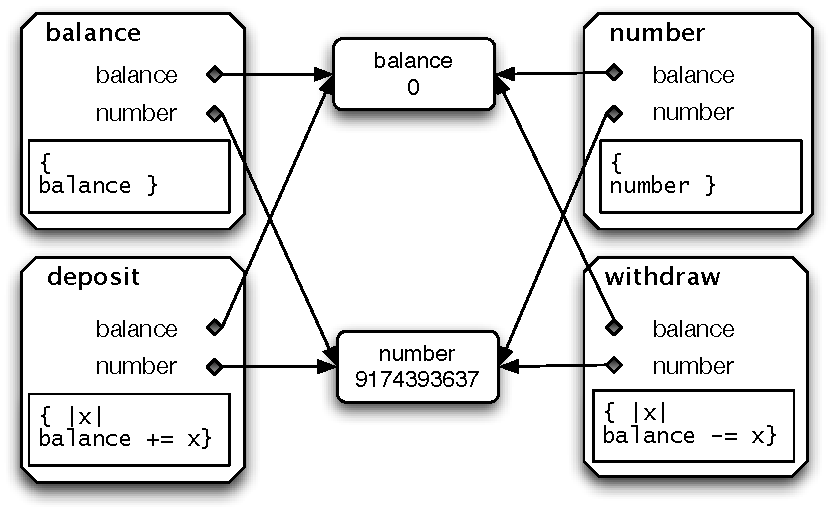
\includegraphics{omnifigs/bank_account_dia}
	}
	\caption{Structure of Bank Account closures}
	\label{fig:bank_account}
\end{figure}

\subsection{Compiled Closures}\label{concepts:compiled_closures}
The TEM is intended to provide trusted execution at commodity prices.
Therefore, the design will be implemented in embedded chips, where persistent
variables are expensive\footnote{Variables' values may change, therefore they would have to be
stored in EEPROM. EEPROM is the slowest and most expensive type of on-chip
memory.}. The following optimization, inspired from \cite{Ste:78b} helps
reduce the amount of shared memory cells used by a closure. Some of the
variable bindings are de-facto immutable (constant). That is, the values of the
bindings will never be modified throughout the lifetime of a closure. This
means that, instead of storing the binding's value in a shared memory location,
the constant value can be stored directly in each closure's binding table. This
eliminates most uses of shared memory locations. \cite{Ste:78b} uses this
mechanism to decide whether frames will be allocated on the stack or in the
heap.

For example, knowing that all the languages used in this section (Scheme, Ruby,
Java) pass primitive types by value (as opposed to passing by reference) allows
us to assert that \texttt{term} in listings \ref{simple_closure:scheme},
\ref{simple_closure:java}, and \ref{simple_closure:ruby} are de-facto
immutable. The proof is quick and straight-forward: \texttt{term} is a
function parameter, therefore it is local to the \texttt{adder} function.
\texttt{fact} is not on the left-hand side of any assignment in \texttt{adder},
therefore it is de-facto immutable.

By a similar argument, it is easy to prove that \texttt{number} in listing
\ref{fig:bank_account} is de-facto immutable, and \texttt{balance} isn't. So
the closures' binding tables can be optimized to use one shared memory location
instead of two, as illustrated in figure \ref{fig:bank_account}.

\begin{figure}[hbtp]
	\center{
		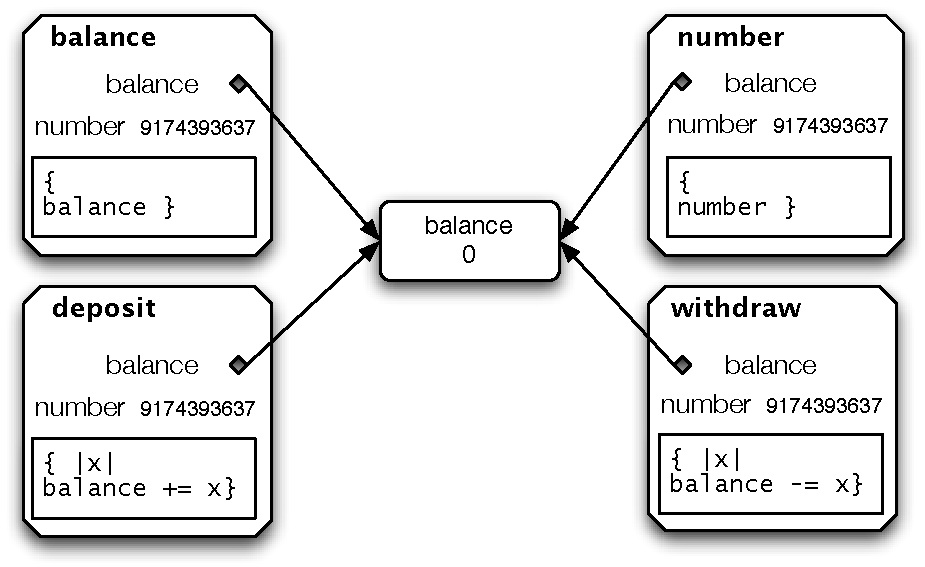
\includegraphics{omnifigs/bank_account_diax}
	}
	\caption{Optimized structure of Bank Account closures}
	\label{fig:bank_account:optimized}
\end{figure}

The result in figure \ref{fig:bank_account:optimized} is further amenable to well-known
optimizations, such as removing the unreferenced entries in the closures'
binding tables. For instance, the variable \texttt{number} is not used at all
in the closures \texttt{balance}, \texttt{deposit}, and \texttt{withdraw}, so
it can be removed from their binding tables.

A \textbf{compiled closure} is a closure that has been fully optimized for the
computer that is intended to execute it. A compiled closure consists of the
following:
\begin{itemize}
  \item the computation to be performed, expressed as executable instructions
  that can be interpreted by the target computer,
  \item a binding table that contains all the non-local variables,
  \item values for the non-local variables that are de-facto immutable, and
  \item addresses (references to shared memory locations) for mutable
  non-local variables.
\end{itemize}

As a note, the approach used in Erlang \cite{carlsson2004cel} deserves interest.
The language has no mutable state, so closures do not need shared memory
locations. This is essential for concurrent programming. Upon further
inspection, I decided that the ideas used to implement mutable state in
Erlang (e.g., Mnesia \cite{mattsson1999mdr}) would prove less efficient than
allowing shared memory cells and using the optimizations described above.


\section{Trusted Execution}\label{concepts:trusted_execution}
This section argues that trusted execution is equivalent to being able to
guarantee the integrity and confidentiality of a computation.

Starting out from an intuitive level, I claim that Yu\footnote{Yes, Yu
is intentionally spelled so that it reads just as \textit{you}.} trusts a
computer if she has confidence that the computer is doing what she expects it
to be doing.

For instance, software developers trust their computers to faithfully execute
their code, and not share it with the outside world. When an issue occurs, the
cause is assumed to be a bug in the program undergoing development, and the
average developer never wonders if the CPU did execute the code it was
given, or if the low-level instructions produced by the compiler or interpreter
match the source code. On the other hand, if the same software developer plays
a game over the Internet and is pwned\footnote{loses dramatically}, the first thought that will come to
her mind will be ``did they use hacks\footnote{modifications to a game's
executable code which help a player perform better by revealing secret
information or improving their commands}?!''

Like most other people, Yu naturally trust computers she owns, and she trusts
the communication between her and a computer in her physical vicinity. However,
when using a system that is not in the same room (for instance, over the
Internet), or a system that belongs to someone else, Yu's trust disappears  as
she is concerned that the computer's owner may tamper with the executable
instructions or the program's data.

The example above highlights two factors that can make Yu distrust the output
produced by a system:
\begin{itemize}
  \item {physical vicinity;} Unless the computer is close to her, Yu doesn't
  trust the communication channel. This problem has been solved, and the
  standardized solutions are SSL \cite{freier1996ssl} and TLS
  \cite{dierks1999tpv}.
  \item {ownership;} Yu does not trust computers owned by others.
  Commodity computers were fundamentally designed to run arbitrary code, and all
  attempts at building systems that restrict the access of owners to their
  computers have failed. (and met with huge amounts of protest)
\end{itemize}

\subsection{Trusting Other People's Computers}\label{concepts:use_model}
The hard (and therefore interesting) scenario is that Yu needs to perform a
computation on Mii\footnote{You are right, Mii was intended to read like
\textit{me}. The name was invented by Nintendo, and is used for player
avatars on the Wii gaming console.}'s machine, and needs the guarantees of
trusted execution. From this we can infer the following:

\begin{enumerate}
  \item {The computation is part of an interaction between Yu and Mii.}
  Otherwise Yu could have run the code on her own computer that she trusts.
  \item {Mii has an incentive to complete the interaction between Yu and Mii.} If
  that is not the case, then Mii has no incentive to run Yu's code on his
  computer, let alone provide trusted execution guarantees.
\end{enumerate}

So the process will be carried out as follows:
\begin{enumerate}
  \item Yu will package the instructions to carry out the computation she
  needs in a format suitable for consumption by Mii's TEM.
  \item Yu will transmit the package to Mii.
  \item Mii will instruct a TEM attached to his computer to execute the
  package.
  \item If Yu needs to know the result of the computation, Mii will transmit
  this result to Yu.
\end{enumerate}

The scenario presented above will be referred to as the use model of the TEM,
because it reflects the way I intend users to interact with the platform.

\subsection{Integrity and Confidentiality}\label{concepts:guarantees}

We start out by defining integrity and confidentiality. Note that the
definitions assume the context of the use model introduced in section
\ref{concepts:use_model}.

\begin{definition*}
Integrity is the guarantee that the computation being carried out on Mii's
computer  is the one specified or intended by Yu.
\end{definition*}

Practically speaking, integrity means that Mii should not be able to change the
computation performed by his computer. Using the bank account example in
section \ref {concepts:closures} (listing \ref{bank_account:ruby}), Yu would be
the online banking provider, and Mii would be an account holder in Yu's bank.
Integrity implies, for instance, that Mii cannot modify the computation in
\texttt{withdraw} so that balance remains unchanged (and thus gain an infinite
amount of money).

\begin{definition*}
Confidentiality is the guarantee that Mii will not learn any information that
is not explicitly disclosed by Yu, as a result of performing the computation.
In other words, Yu's secrets will be shielded from Mii.
\end{definition*}

As an initial motivation for confidentiality, note that computer systems are
used in a competitive society, so it is unavoidable that computations will
involve information that should be shielded from some parties.

The rest of this section relies on the intuition and the use model developed so
far to prove that trusted execution is equivalent to the guarantees of integrity
and confidentiality. First, I prove that integrity is required by trusted
computing, then I prove that integrity requires confidentiality. The proofs
also show how that trust in execution can be asserted based on given integrity
and confidentiality.

\begin{theorem*}
Trusted execution requires the guarantee of integrity.
\end{theorem*}

\begin{proof}
The use model described in section \ref{concepts:use_model} is assumed. All
scenarios where the TEM use model holds can be classified into of the following
categories:
\begin{enumerate}
  \item {the computation contains one of Yu's secrets}, so integrity is
  required, to ensure that the computation isn't transformed in a way that
  would make the result give Mii information about Yu's secrets (e.g., replace
  the entire execution with ``\texttt{return \textit{secret}}'').
  \item {the computation does not act on any of Yu's secrets}, so it must be
  the case that Mii will contribute some information to the computation, and
  that Yu needs to trust the final result. If Mii has no contribution, then
  Yu can execute the computation on her own computer which she trusts. If Yu
  does not need to trust the final result, it follows that Mii is the only one
  using the result, therefore Mii can obtain Yu's information (which contains
  no secrets, according to the hypothesis for this category) and execute it on a
  computer that Mii alone trusts. This contradicts the hypothesis that trusted
  execution (as defined in at the beginning of the section) is needed.
\end{enumerate}
\end{proof}

\begin{theorem*}
The integrity guarantee of trusted execution requires confidentiality.   
\end{theorem*}

\begin{proof}
Assume that the computation to be performed does not require any secret that
Mii does not posess. Otherwise, confidentiality is trivially required, because
the computation's specification includes the requirement of not disclosing the
secrets.

The Church-Turing thesis (explained in \cite{kleene1952im}) holds for today's
computers. This has the implication that a very simple computer (a Turing
machine) can emulate any commodity computer that has been built to date. Since
all computers can essentially perform the same calculations, it follows that it
is impossible for Yu to formulate her computation in such a way that carrying
out the computation on different computers would yield different results. Thus,
Yu cannot distinguish between the case where Mii would show her the
genuine result of her computation, and the case where Mii would show her
maliciously contrived data.

We conclude that if the computation doesn't depend on information that is
secret from Mii, no proof of integrity can be built. Conversely, proving
integrity requires information that is secret from Mii, so confidentiality is
required to ensure that the information stays secret from Mii.
\end{proof}


\section{A Chain of Trust for the TEM}\label{concepts:trust_chain}

Section \ref{concepts:guarantees} shows that trusted execution requires that a
secret be established between Yu and Mii's computer that Yu trusts. This
section describes a chain of trust that allows Yu to assert that a public key
corresponds to a private key that can only be found inside a computer Yu
trusts. The chain of trust was derived by removing the unnecessary parts from
the chain of trust used for platform attestation in the TPM \cite{tcpa2007}.

\begin{figure}[bhp]
	\center{
		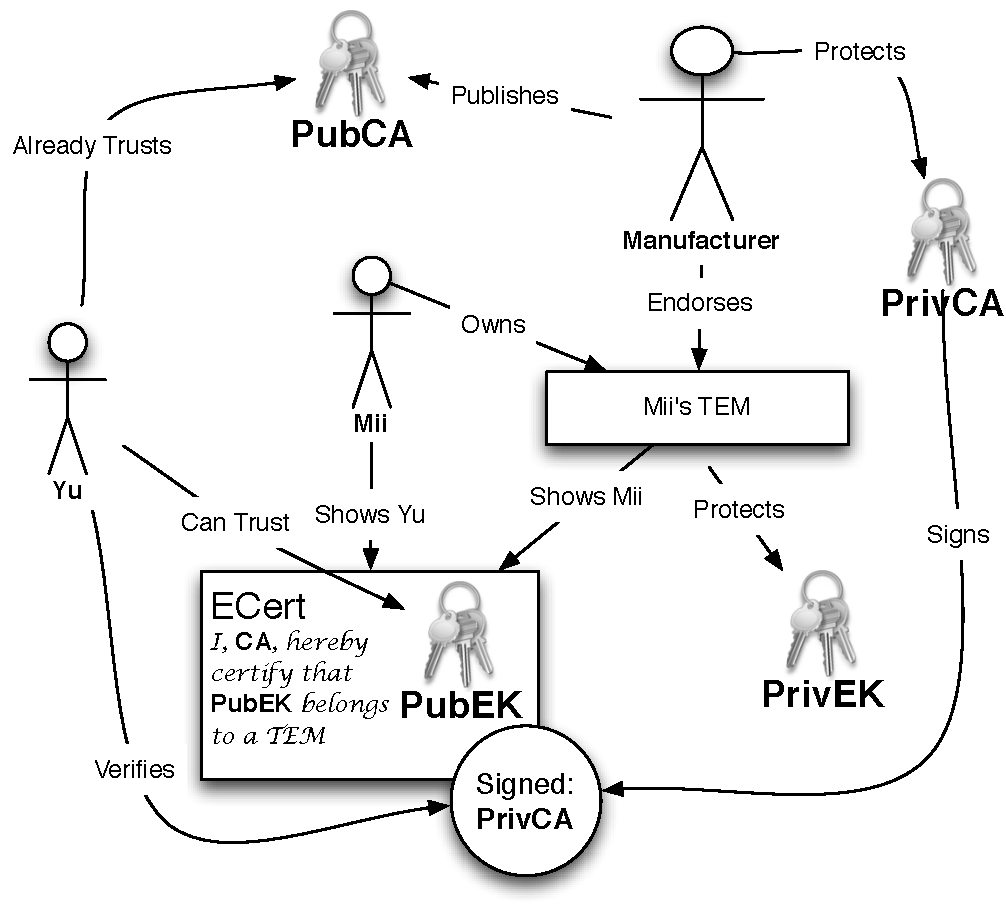
\includegraphics{omnifigs/trust_chain}
	}
	\caption{The Chain of Trust Used by Yu to Trust the TEM }
	\label{fig:trust_chain}
\end{figure}

The public and private keys in this section can use any public-key encryption
system, such as RSA \cite{rivest1978mod} or ECC \cite{koblitz1987ecc}. Figure
\ref{fig:trust_chain} illustrates the chain of trust.

The root of trust is a hardware manufacturer (such as Infineon or Atmel), which
acts as a Certificate Authority in a public key infrastructure as defined in
\cite{housley2002ixp}. The manufacturer has an asymmetric key named the
Certificate Authority key. This key consists of protects the private key
(PrivCA), while the public key (PubCA) is assumed to be well known.

At TEM manufacturing time, an asymmetric key, called an Endorsement Key,
is generated for each TEM. The Private Endorsement Key (PrivEK) is securely
embedded into the TEM. Then the manufacturer's private key (PrivCA) is used to
sign an Endorsement Certificate (ECert) containing the TEM's Public
Endorsement Key (PubEK), and stating that the Endorsement Key has been embedded
in a hardware device that provides the security guarantees required by a TEM.

The TEM's Public Endorsement Key can be used to encrypt a secret generated
by Yu, which becomes the shared secret between Yu and Mii's TEM needed to
satisfy the requirement in \ref{concepts:guarantees}. Once Mii presents Yu with
his TEM's Endorsement Certificate, she is assured that any secrets encrypted
with PubEK can only be decrypted by Mii's TEM, as it is the only computer that
knows PrivEK. This method allows for secret information to flow securely from
Yu to Mii's TEM. If there is a need for secret information to flow the other
way, Yu can send Mii's TEM a symmetric\footnote{Building symmetric encryption
features into the TEM requires careful consideration, because most countries
regulate the use of symmetric encryption algorithms.} or
asymmetric encryption key, which is protected as described above, and allows for secure
communication of secrets in both directions.

As stated towards the beginning of this section, the chain of trust is rooted
at the hardware manufacturer who emits the Endorsement Certificate. Readers
troubled by the need to trust big manufacturers should note that they have
probably entrusted their information to small stores and credit unions, as well
as to people working for various institutions.

\subsection{Anonymizing the TEM}\label{concepts:anonymous_trust}
The chain of trust above has a potential issue: the proof that a TEM can be
trusted requires the Public Endorsement Key. Since a TEM has exactly one PubEK,
the PubEK can be used to identify and track the TEM, and thus its owner. This
may be unacceptable in some circumstances, as it leaks information about the
users' identity, just like the Intel Processor Serial Number (PSN)
\cite{gengler1999isi}, which has generated great public uproar. Fortunately,
the chain of trust described above can be amended in a way that makes the TEM
untraceable.

The threat to anonymity stems from the fact that a TEM has a single Public
Endorsement Key, which acts as a shared secret between the TEM and Yu, so Yu
sees the same PubEK every time she interacts with Mii's TEM. This can be
improved by adding an extra layer of keys, as follows.

In the modified design, when Mii needs to interact with Yu, he instructs his
TEM to create a new asymmetric User Key, which is handled similarly to the
Endorsement Key. The Private User Key (PrivUK) is never disclosed by the TEM,
and the Public User Key (PubUK) is included in a User Certificate (UCert)
signed by the TEM's Private Endorsement Key (PrivEK). The User Certificate
states that the User Key was generated by the TEM, and the appropriate security
guarantees hold.

Mii sends the User Certificate, together with the Endorsement Certificate, to a
trusted server maintained by the TEM's manufacturer. The server verifies the
two certificates to make sure that the Public User Key was indeed generated by
a TEM emitted by the manufacturer, then the server gives Mii a User Endorsement
Certificate (UECert) signed by the manufacturer's private CA key (PrivCA), and
stating that the User Key provides all the security guarantees of a TEM User Key.

At the end of the process Mii can use the User Endorsement certificate to prove
that the User Key can be trusted just as much as an Endorsement Key. However,
UECert does not contain any information identifying the particular TEM used to
generate the User Key. So this mechanism makes the TEM untraceable.

The process described in this section does not require any special-purpose
mechanism in the TEM. The steps above can be implemented in the TEM as programs
on top of the architecture presented in chapter \ref{arch}, which was designed
without regard to this section. Therefore, the information here does not
pertain to the TEM's design. Rather, it is included as to pacify any anonymity
concerns that a reader may have.

\section{Security-Enhanced Closures}\label{concepts:secure_closures}

Section \ref{concepts:closures} states that the closure is the execution
primitive of the TEM, and illustrates the structure of a closure. It follows
that the TEM's mission is to provide trusted execution for closures.
According to section \ref{concepts:guarantees}, this is equivalent to
guaranteeing integrity and confidentiality.

Section \ref{concepts:information_classes} classifies the information
inside a closure as \textit{private}, \textit{shared}, or \textit{open},
according to the guarantees needed. A \textbf{Security-Enhanced Closure (SEClosure)}
is a closure with all the information classified as described above.

Before they can be executed by the TEM, SEClosures must be compiled and encoded in a format that is easy to process, so that the logic to be implemented inside the TEM is minimized. The rest of this work uses the term \textbf{SECpack} to refer to compiled and encoded SEClosures.

SECpacks are suitable to be executed by the TEM, but the information inside
them is unprotected. Section \ref{concepts:secpack_binding} describes a
process that uses a TEM's Public Encryption Key (PubEK) to produce a
\textbf{bound SECpack}. The bound SECpack contains the same information as the
original SECpack, but it enforces the confidentiality and integrity of the
information it contains. Thefore, Yu can safely give Mii a SECpack that was
bound to Mii's TEM. The term \textit{bound} is justified by the fact that a
bound SECpack can only be used by the TEM whose PubEK was used to produce the
bound SECpack.

\subsection{Security Guarantee Classes}\label{concepts:information_classes}

Section \ref{concepts:guarantees} shows that trusted execution is equivalent
to providing integrity and confidentiality guarantees. However, both guarantees
are not needed by all the information expressing a computation. Therefore it
makes sense to classify the information, according to the guarantees needed:
\begin {itemize}
  \item \textbf{private}: this is information that requires the confidentiality
  guarantee. Examples of secret information are Yu's social security number, or
  one of her private encryption keys.
  \item \textbf{shared}: this is information that only requires an integrity
  guarantee. In the back account example in section \ref{concepts:closures}, if 
  the code for \texttt{withdraw} can be changed to the code for
  \texttt{deposit}, that would have dramatic consequences on the bank.
  \item \textbf{open}: this information is not covered by any guarantee. This
  has to be information that Mii supplies to the computation. As described in section
  \ref{concepts:use_model}, Mii is the TEM's owner, and therefore he is the only
  one who would trust the platform automatically, without requiring any proof
  of integrity or confidentiality.
\end{itemize}

Private information must automatically receive an integrity guarantee, in order
to ensure no secret is leaked. For example, secrets are usually encryption or
signing keys. If Mii can replace one of Yu's key with his own, Yu's key will
still be confidential, but Mii can access any information encrypted by Yu's key.

Section \ref{concepts:guarantees} proves that all the executable code in a
closure requires an integrity guarantee. It follows that for trusted execution,
all the executable code in a SEClosure is either private or shared.

For reasons of simplicity, it seems appealing to remove the \textit{shared}
class of information, and specify that all the information originating from Yu
is private. However, if all the executable code is made private, then it is
impossible for Yu to prove Mii anything about the nature of the computation
expressed in the closure. The shared class is motivated by my conviction that
known information should not be encrypted, and by applications where Mii must
verify that the closure expresses a certain computation.

The next section describes a method for implementing the security guarantee
classes presented here, thus demonstrating that the idea is practical.

\subsection{Implementing the Security Guarantee
Classes}\label{concepts:secpack_binding}

The TEM's use model (section \ref{concepts:use_model}) states that the
information describing Yu's computation will pass through at least one
intermediary (Mii) before reaching the TEM. Therefore, it is reasonable to
assume that the information can be altered arbitrarily in the passage from Yu
to Mii's TEM.

Fortunately, Yu can be assumed to know the TEM's Public Endorsement Key
(PubEK), and she can use it to communicate secrets securely to the TEM,
according to section \ref{concepts:trust_chain}. The following process,
illustrated in figure \ref{fig:secpack_binding}, uses the Public Endorsement Key to
convert a SECpack into a form that provides the appropriate guarantees (section
\ref{concepts:information_classes}) for the information inside the SECpack,
despite the fact that the information has to pass through Mii's hands.

\begin{figure}[hbtp]
	\center{
		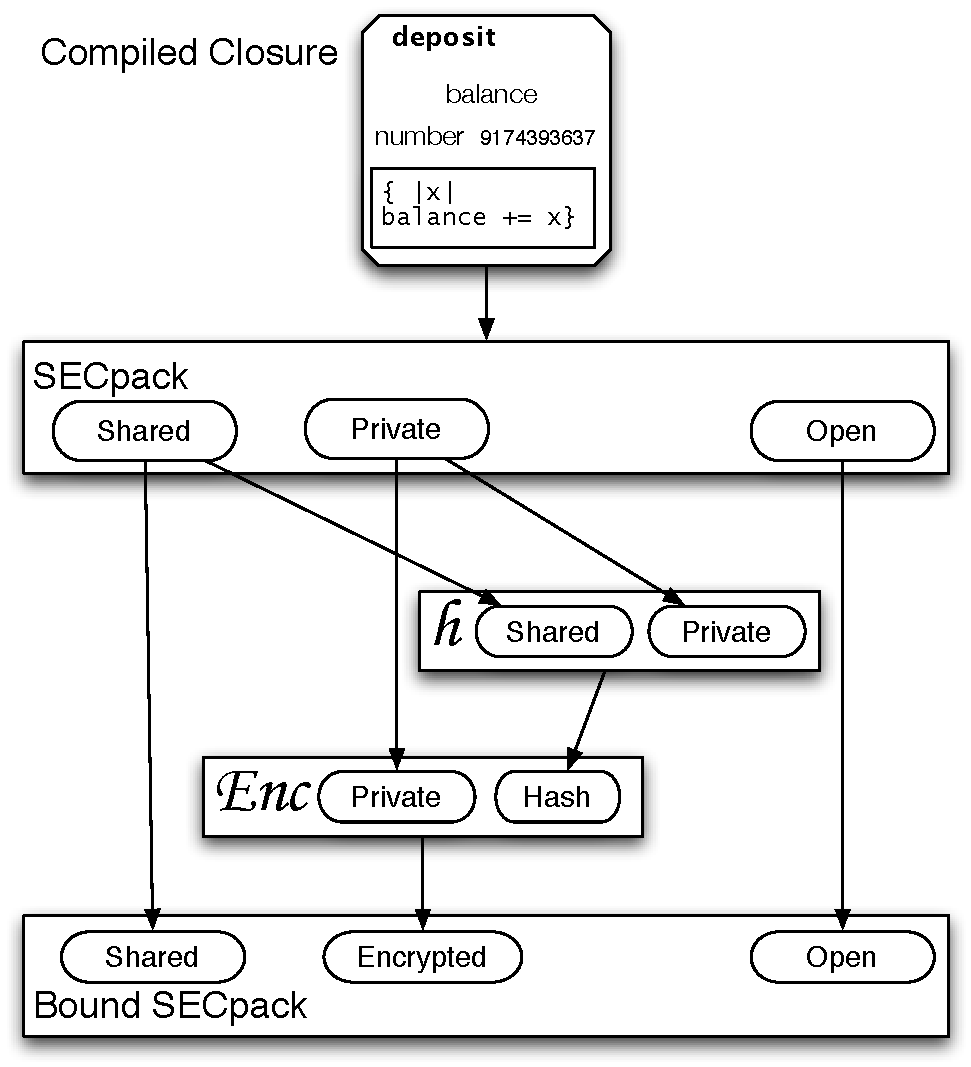
\includegraphics{omnifigs/secpack_binding}
	}
	\caption{Securing the Information in a Closure}
	\label{fig:secpack_binding}
\end{figure}


\begin{enumerate}
  \item Let $\mathcal P$ be the private information, $\mathcal S$ be the shared
  information, and $\mathcal O$ be the open information.
  \item Use a cryptographic hashing function $h$ (such as SHA1
  \cite{eastlake2001rus} or MD5 \cite{rivest1992rmm}) to compute a message
  digest of the private and the shared information. $$\mathcal H = h(\mathcal P
  || \mathcal S)$$ Note: $||$ denotes concatenation.
  \item Use the TEM's Public Endorsement Key to encrypt the private information
  together with the message digest. $$\mathcal E =
  {\mbox{\Large \textit{Enc}}}_\textrm{PubEK}\Big(\mathcal P || \mathcal
  H\Big)$$
  \item The secured closure consists of the encryption result $\mathcal E$,
  together with the shared information $\mathcal S$, and the open information
  $\mathcal O$. $$\textrm{Secured Closure} = (\mathcal S || \mathcal E ||
  \mathcal O)$$
\end{enumerate}

Yu will follow the process above to secure her closure before transmitting it
to Mii. When Mii's TEM will receive the closure, it will use its Private
Endorsement Key (PrivEK) to decrypt $\mathcal E$ and obtain $\mathcal P$ and
$\mathcal H$. In order to guarantee integrity and privacy, the TEM will refuse
the input if $\mathcal H$ doesn't match the hash of $\mathcal P || \mathcal S$.
This is sufficient to provide the security guarantees for private and shared
data, as proven by the following:

\begin{theorem*}
The scheme described above guarantees the confidentiality of the
private information $\mathcal P$ and the integrity of the shared information $\mathcal S$ and
the private information $\mathcal P$.
\end{theorem*}
\begin {proof}
By strong induction over $N_E$, the number of execution attempts of the secured
closure on Mii's TEM. Note that an execution attempt can fail, if Mii attempts
to change $\mathcal P$ and/or $\mathcal S$ in the closure (the fact follows
immediately from this theorem).

\textbf{Base case.} the guarantees are provided on the secured closure's first
execution attempt.

$\mathcal P$ cannot be directly derived from $\mathcal E$, assuming the
encryption algorithm associated with PubEK is resistant to Mii's
attacks\footnote{This is believed to be true, at least
for RSA \cite{rivest1978mod} and ECC \cite{koblitz1987ecc}.}, and that $h$ is
inverse-resistant\footnote{It is impossible to compute $\mathcal P || \mathcal
S$ from $H$. This is true for any good cryptographic hash function, and it is
believed to be true for SHA1 \cite{eastlake2001rus} and MD5
\cite{rivest1992rmm}.}. As a special case, note that $\mathcal P$ will never be
empty, because the trusted execution assumption implies the existence of
confidential information, as proven in section \ref{concepts:guarantees}.

Assuiming $\mathcal P$'s confidentiality (proven above), it follows that, in
order for Mii to mutate $\mathcal S$ to $\mathcal S'$, Mii must break $h$ as
well as ${\mbox{\Large \textit{Enc}}}_\textrm{PubEK}$ in order to produce
the correct values of $\mathcal H'$ and $\mathcal E'$ without knowing
$\mathcal P$.

The process is resistant to modifications of $\mathcal P$
as well, as long as the entire value of $\mathcal P$ is not replaced. Assume
the mutation transforms $\mathcal P = (P_\alpha || P_0 || P_\Omega)$ into
$\mathcal P' = (P_\alpha || P_1 || P_\Omega)$. The argument in the previous
paragraph can be used to show that Mii must break $h$ and ${\mbox{\Large
\textit{Enc}}}_\textrm{PubEK}$, since he does not know $P_\Omega$ and/or
$P_\alpha$ (at most one of them may be empty).

Therefore, Mii cannot determine his TEM to execute the secured closure with
modifications to $\mathcal P$ or $\mathcal S$ without replacing $\mathcal P$
completely. But once $\mathcal P$ is replaced with a value known by Mii, the
closure does not contain any of Yu's secrets. Therefore, the notion of trusted
computation isn't applicable to the resulting closure -- the computation in it
can be specified by Mii alone, and executed on any platform.

\textbf{Induction step.} assuming the guarantees are provided on the secured
closure's first $N_E$ execution attempts, I will prove that the guarantees will
be provided on the $(N_E + 1)^\textrm{th}$ attempt.

$\mathcal P$'s integrity is guaranteed for attempts $1 \ldots N_E$, so the TEM
cannot be used to execute closures containing arbitrary mutations of $\mathcal
P$. Therefore, no information about $\mathcal P$ is leaked in the first $1
\ldots N_E$ attempts. Hence, recovering $\mathcal P$ on the $(N_E +
1)^\textrm{th}$ attempt is just as difficult as recovering it directly from $\mathcal E$.
Therefore, the assumptions of the base case still hold, and the same argument
can be used for the induction step.
\end{proof}

\section{Persistent Store}\label{arch:pstore}
The persistent store is an associative memory backing the values of
mutable non-local variables for all the closures executing on the TEM. Section
\ref{concepts:pstore} argues that the most appropriate design is to identify
variables by addresses that are as large as cryptographic hashes, and use the
knowledge of a value's address as proof of authorization to access that
variable.

The conceptual presentation of the persistent store leaves out the following
issues:
\begin{itemize}
  \item the operations supported by the persistent store,
  \item the nature of the values in the store,
  \item the method for assigning an address to a variable, and
  \item bridging the gap between the possibility of executing a large number of
  SECpacks, and the small amount of non-volatile memory in the low-cost secure
  chips that the TEM targets.
\end{itemize}
The omission is deliberate, as the answers to these questions are engineering
trade-offs, and would have detracted from the understanding of the concept. This
section provides answers that are appropriate in the context of the TEM
architecture.

\subsection{Persistent Store Operations}
In the absence of a contrary reason, the persistent store provides the standard
associative memory operations:
\begin{itemize}
  \item \texttt{read(address)} returns the value stored at \texttt{address}, or
  a special \textsc{nothing} value if the persistent store does not have an
  association for the given address.
  \item \texttt{write(value, address)} writes \texttt{value} at
  \texttt{address}. \texttt{write} overwrites the old value stored at the given
  address, or creates a new association for \texttt{address}, and returns
  \textsc{created} or \textsc{updated} to reflect what happened. The return
  value is not relevant for a general understanding of the TEM archiecture, but
  it is needed in section \ref{arch:pstore_external}.
  \item \texttt{remove(address)} removes the value associated with
  \texttt{address}, if such an association existed.
\end{itemize}

\subsection{Persistent Store Values}
All the values in the TEM's persistent store are the size of the hashes
produced by the TEM's cryptographic engine (section \ref{arch:crypto_hash}).

Using fixed-size variables is essential to avoid complexity in the persistent
store implementation. Furthermore, an implementation that provides
variable-size values will end up using most (if not all) of the saved memory on
the bookkeeping required to make variable lookup fast.

The reasoning behind the chosen size requires some understanding of the TEM's
execution engine, described in section \ref{arch:execution}. The unique memory
space and the stack-based instruction set suggest a single attractive
alternative to the choices of value size: the size of a machine word. This
choice would make programming a bit more convenient, because it would be
possible to read a persistent store value directly onto the stack, or write
calculation results directly from the stack to the persistent store.

However, word-sized values  would cause memory waste, because a persistent
store value would be much smaller\footnote{The chips suitable for the TEM at
the time of this writing have a word size of 16 bits, whereas a SHA-1 hash
takes 160 bits.} than its address, so most of the memory would be spent on
addresses.

Furthermore, larger persistent store values can translate into speed benefits.
Closure compilers can bundle multiple variable values into the same persistent
store entry, in order to optimize speed. This will always yield benefits,
because reading/writing from/to the persistent store implies NVRAM, and
therefore is bound to be slower than multiplexing values in a closure's
RAM-backed memory space.

In conclusion, making persistent store values approximately the same size
as addresses makes sense for the TEM. The slight increase in complexity for the
closure compiler is rewarded by increased SECpack execution speed, and
better memory utilization.

\subsection{Persistent Store Address Allocation}\label{arch:ps_alloc}
The size of persistent store addresses must be at least as large as a symmetric
encryption key (section \ref{concepts:pstore}). This allows the following
allocation strategy: randomly choosing a persistent store address allocates that
address on all the TEMs in the world. Address allocation is used to mean that
no other closure will use the same address for a different variable. Address
allocation does not imply memory allocation on any TEM.

This strategy has the advantages that a variable has the same address on all
TEMs, and that address allocation can be done off-line. On the other hand, the
method's robustness is not immediately obvious, and guaranteeing integrity
against replay attacks is non-trivial. An argument for the method's robustness
is provided below. The discussion on preventing replay attacks is complex
enough that it has been assigned to its own section \ref{arch:pstore_freshness}.

\subsubsection{Robustness Argument}
Allocating an address uses the same mechanism as generating a symmetric
encryption key. Addresses are large enough that the chance of a conflict is not
bigger than the chance of generating an encryption key that belongs to someone
else. Most of the world's economy relies on symmetric encryption, as banks
communicate with each other using SSL \cite{freier1996ssl} or TLS
\cite{dierks1999tpv}, which in turn use symmetric encryption.

An argument similar to that in section \ref{concepts:pstore_auth} can be
used to show that the probability of having an attacker break the TEM trust
chain is much greater than the probability of having two SECpacks on the same
TEM that use the same address for different variables.

In closing it is worth noting that increasingly many systems rely on UUIDs
(Universally Unique Identifiers) \cite{leach2005ruu} for what is
essentially off-line address allocation. Using a hardware random number
generator to allocate a persistent store address is stronger than
the pseudo-random UUID allocation algorithm proposed in \cite{leach2005ruu}.
It is assumed that a SEClosure author has access to a good hardware RNG.

\subsection{Guaranteeing the Freshness in the Persistent
Store}\label{arch:pstore_freshness}
Guaranteeing freshness when the persistent store addresses are allocated 
offline requires some thought. It is non-trivial for a SEClosure to distinguish
between the case when its mutable non-local variables have never been used on a
TEM (and thus should be assumed to contain default values), and the case when
its variables have been assigned values, but the corresponding associations
have been \texttt{remove}d from the persistent store. The possibility of
confusing the two cases can be exploited by replay attacks.

\subsubsection{Preventing Replay Attacks: the Easy Way}
The straightforward method of eliminating the ambiguity is to specify
that once a persistent store association is created, it persists for the
lifetime of the TEM. In other words, the operation \texttt{remove} is forbidden.

When adopting this solution, the following concerns need to be addressed:
\begin{itemize}
  \item the persistent store grows proportionally to the number of
  non-local mutable variables used by SECpacks throughout the life of the TEM,
  and
  \item malicious SECpacks can initiate a denial of service attack by filling
  up the persistent store.
\end{itemize}

However, this solution is easier to understand and implement, so it may be more
desirable in some situations. All off the issues above can be worked around.

The persistent store entries can be stored in untrusted memory (as explained in
section \ref{arch:pstore_external}), and the capacities of both hard disks and
flash memories has been increasing at a rate that exceeds Moore's law. Denial of
service attacks can be prevented by placing a hard limit on the number of new
persistent store variables can be used by a SECpack.

\subsubsection{Preventing Replay Attacks: the Painful but Efficient Way}
The method of preventing replay attacks explained above is easy to understand,
but has a potential drawback in that all the non-local mutable variables
used on a TEM must persist forever, even if the SECpacks referencing them
will never be executed again. This section describes a more complex method for
preventing replay attacks that allows unused values to be \texttt{remove}d from
the TEM. The presentation requires a significantly deeper understanding of the
TEM as a whole, and is not as self-contained as the previous section.

The problem of preventing replay attacks can be reduced to avoiding the replay
of the initialization of the persistent store variables. This is because normal
SECpacks assume that the relevant mutable non-local variables have been
initialized prior to execution, so persistent store \texttt{read}s will never
return \textsc{nothing}. If this assumption is broken, a SECpack aborts its
execution and does not return any information  o the TEM owner. 

The only computation that is vulnerable to replay attacks is now the
initialization of persistent store variables. At-most-once semantics can be
provided for initializations by linking them to a monotonic counter inside the
TEM. This approach requires that a single value, the monotonic counter, has to
persis throughout the lifetime of the TEM. The rest of the section explains
the idea in more detail.

Let an \textbf{object}\footnote{Object-Oriented Programming is used to simplify
the presentation. However, the mechanism presented here can be easily
adapted to other programing paradigms.} be a group of SECpacks that use the
same mutable non-local variables. For convenience, an object's \textbf{fields}
shall be all the mutable non-local variables used by the SECpacks in the
object. Using the bank account example in section \ref{concepts:closures}, an
individual bank account is an object, and it consists of the SECpacks labeled
\texttt{withdraw}, \texttt{deposit}, \texttt{balance}, and \texttt{number}. The
bank account has one field, the variable \texttt{balance} (\texttt{number} is
optimized away by the closure compiler because it is de-facto immutable).

To reduce complexity, the lifetime of all the fields of an object are managed
at once, and management follows the same principles as constructors and
destructors (also named finalizers). Namely, an object is \textbf{constructed}
on a TEM by assigning initial values to all its fields. An object is
\textbf{destroyed} by \texttt{remove}-ing the values of its fields from the
persistent store. The SECpacks in an object will abort execution if any of
the fields they reference do not have a value in the persistent store,
because that means the TEM owner destroyed the object prematurely.

\subsubsection{Preventing Replay Attacks on Object Construction}
The solution is completed by ensuring that an object is constructed at most
once. A simple mechansim that achieves this goal is described below.

The mechanism uses a single monotonic counter, $\mathcal{M}_C$. The monotonic
counter's value is stored in the persistent store, at an address known only to
privileged SECpacks (described in section \ref{arch:key_store}). 

Constructing an object is achieved series of assignments to persistent store
addresses. The object's owner can construct a list of (address, value) tuples
that completely capture this information. This list is referred to as the
\textbf{constructor table}. 

Yu follows the following steps to produce an object that Mii can use on his
TEM:
\begin{enumerate}
	\item Mii runs a privileged SECpack that returns the value of
	$\mathcal{M}_C$, signed with the TEM's Private Endorsement Key, $r_v =
	\mathcal{M_C} || Enc_\textrm{PrivEK}(h(\mathcal{M}_C))$.
	\item Mii gives Yu $r_v$, the result of reading the
	counter, together with the TEM's Endorsement Certificate.
	\item Yu verifies ECert and the signature, to make sure that
	the Public Endorsement Key in the certificate can be trusted, and that
	the value of $\mathcal{M}_C$ is authentic.
	\item Yu binds the object's SECpacks to the TEM using PubEK,
	and also encrypts the \textbf{constructor data}, which is the constructor table
	together with the value of $\mathcal{M}_C$ that was verified in the previous step. The results produced
	at this step are given to Mii.
	\item Mii runs a privileged SECpack that decrypts the constructor data using
	PrivEK, and verifies that the value of $\mathcal{M}_C$ matches the value in
	the constructor data. If the verification is completed, then the SECpack
	carries out the \texttt{write}s described in the constructor table, and
	increments $\mathcal{M}_C$.
\end{enumerate}

It is easy to see that the process above does not allow an object
to be constructed twice -- exactly one object is constructed for a certain
value of $\mathcal{M}_C$. Guaranteeing that Mii cannot replay the constructor
assignments translates into guaranteeing freshness for the fields of an
object, which are, by definition, all the values that SECpacks will read
from the persistent store.

\subsection{Secure External Memory: The World in a
Nutshell}\label{arch:pstore_external}
Section \ref{concepts:pstore} explains that the persistent store must protect
its contents from attempts of bypassing the associative memory interface.
This leads to the straightforward implementation of storing all the
associations in non-volatile memory shielded by the TEM's tamper-resistant
envelope. Unfortunately, secure NVRAM is expensive, so it does not come in
abundance on the low-cost chips that the TEM targets. This section analyzes the
possibility of using untrusted memory outside the TEM's secure envelope, which
is significantly less expensive.

The TEM uses the approach to external secure memory introduced by the AEGIS
\cite{suh2003aat} secure processor, which leverages Merkle trees
\cite{merkle1980ppk}. The persistent store's external memory design adapts the
maintainance algorithms to the TEM scenario (a low-cost chip attached to a
powerful, but untrusted processor), and modifies the design slightly to obtain a
hash tree whose height is logarithmically proportional to the number of
associations inside the TEM, and not to the size of the addressing space.

Like AEGIS \cite{suh2003aat}, the persistent store relies on building a tree,
where the leaves store the actual associations, and internal nodes store a
cryptographic hash of their children\footnote{Optimized designs that allow
internal nodes to store associations together with the hash of their children are
reasonably straightforward.}. The tree's root must be stored in NVRAM inside the
TEM's secure envelope, but all the other nodes can be stored in untrusted memory.

In order to ensure the integrity and confidentiality of the data, neither the
persistent store addresses nor the values can be stored ``in the clear'' in
untrusted memory. A symmetric encryption key\footnote{The symmetric
key never leaves the TEM, and can be generated cheaply using a PUF
\cite{gassend2002spr}. }\footnote{If the law does not allow symmetric encryption, an asymmetric key is used instead. Note that the persistent store becomes painfully inefficient in this case.} that is also stored inside the TEM's NVRAM is used to encrypt the associations. The
two parts of an association must be encrypted individually, so that the TEM can
later ask for an association by its encrypted address. This external
representation is used for computing the hashes in the internal nodes, so the
contents of the internal nodes are not confidential.

The TEM's host (with a powerful but untrusted processor) is responsible for
maintaining the tree structure. When a persistent store \texttt{read} is
issued, the TEM communicates the encrypted persistent store address to the
host. The host responds with the encrypted value associated with the
address, together with a proof of correctness consisting of the contents of all
the intermediary nodes. A \texttt{write} is handled similarly, except that the
correctness proof also describes the updates that must be performed to the
tree.

\subsubsection{Amnesia and Replay Attacks}
The tree used for external memory storage is said to exhibit
\textbf{amnesia} if it is possible for the TEM's host, who is managing the tree,
to ``forget'' about a persistent store association. The host would tell the
TEM that an entry does not exist, when in fact it does. Assuming the persistent
store implementation mistakenly believes the owner, the net result would be
that a \texttt{read} could return \textsc{nothing} when it should return a
value, and a \texttt{write} could return \textsc{created} instead of
\textsc{updated}.

An external memory tree exhibiting amnesia is \textbf{acceptable} if the
persistent store design, as a whole, can be used to detect the wrong answers
that can be originated by amnesia and report that the external tree has been
compromised.

Amnesia is important for the persistent store design. External
memory trees that are guaranteed to either provide the correct answer or
exhibit amnesia have a much simpler structure than trees that must provde the
correct answer, without the possibility of amnesia. If amnesia is not
acceptable, then the external tree sturcture must allow the TEM's host to
construct a prof that a tree contains no association for a given address. On
the other hand, if amnesia is allowed, then the host computer can structure the
tree as it wishes, and it does not need to provide a proof when claiming that
the tree does not contain any association for a certain address.

A necessary, but not sufficient, condition for amnesia to be acceptable is that
the correct return value of a \texttt{write} (\textsc{created} or
\textsc{updated}) is known in advance. In other words, whenever a variable is
assigned a value, the persistent store should know whether the store already
contains a corresponding association or not. Otherwise, the host can trick the
TEM into creating two leaves for the same association, and later lead the TEM
to the leaf corresponding to a stale value.

The method of guaranteeing persistent store freshness (section
\ref{arch:pstore_freshness}) determines if amnesia is acceptable. For example,
the straigthforward method described at the beginning of section
\ref{arch:pstore_freshness} requires the guarantee that the persistent store
will not exhibit amnesia, because its correctness relies on receiving the
correct answer from \texttt{read}, and amnesia means that a \texttt{read} may
return \textsc{nothing} when it shouldn't.

On the other hand, the more complicated method described in the same section
works correctly even when faced with amnesia, because it must work correctly
even when the TEM owner \texttt{remove}s associations (intuitively, amnesia
resembles spurious \texttt{remove}s.) The complicated method works correctly
becauseit is known that all the SECpacks of an object will issue only
\texttt{writes}s that return \textsc{updated}, and only \texttt{reads} that do
not return \textsc{nothing}. Also, all the \texttt{write}s in a constructor
are guaranteed to return \textsc{created} under normal use, but this condition
does not need to be verified to insure the correctness of the persistent store
operations.

\subsubsection{Preventing Amnesia}
If the persistent store is not allowed to exhibit amnesia, the host must be
able to prove that an association does not exist in the tree. In order for the
proof to have an efficient encoding (i.e., not enumerate all the leaves in the
tree), there must be a single possible path from the root to a leaf containing
a certain address.

The fixed tree in AEGIS \cite{suh2003aat} trivially meets the requirement
above, but is not ideally suited for a sparse addressing space, because its
height is proportional to the number of bits in an address. The issue is
exacerbated by the pressure of the low-memory TEM environment on the
tree's branching factor. For example, assuming SHA1 is used for
hashing, a branching factor of 1,000 would require 20KB of RAM for storing a
single internal node. 20KB is a luxury in the low-cost chips that the TEM is
targeting. On the other hand, using a really small branching factor increases
the tree depth and lowers performance.

A binary search tree is an attractive alternative, especially because the tree
\emph{does not have to be balanced}. Intuitively, it is safe to assume that the
tree will perform according to the average-case analysis, because the tree keys
are encrypted addresses, so they will ``look'' random. Formally, a misbehaving
SEClosure cannot cause the persistent store to produce a worst-case tree structure, because it cannot guess the addresses that would encrypt to keys that would lead to the worst-case tree structures.

Implementing the binary search trees requires that internal nodes would have to
be augmented to also store addresses, which is straightforward. An optimized
implementation will tweak the tree's branching factor to achieve a good
compromise between the size of an internal node and the tree's height.

%\section{The TEM's Threat Model}\label{concepts:threat_model}


\chapter{Architecture}\label{arch}
This chapter proposes an architecture for the Trusted Execution Module. The
design is driven by the goal of making it possible to manufacture the TEM at very low
cost, which is required if the TEM is to become a commodity. The text in this
chapter makes heavy use of the concepts presented in chapter \ref{concepts}. My
design was probably biased by the prototype implementation on the JavaCard
platform, so it is likely that some of the details will change if the TEM is
implemented directly on a hardware chip.

The main components of the TEM are the execution engine, the cryptographic
engine, and the persistent store. Figure \ref{fig:tem_overview} contains the
(obligatory) block diagram for the platform. The grayed out components are
not mandatory, but their presence can optimize various aspects of the TEM's
functionality.

\begin{figure}[hbtp]
	\center{
		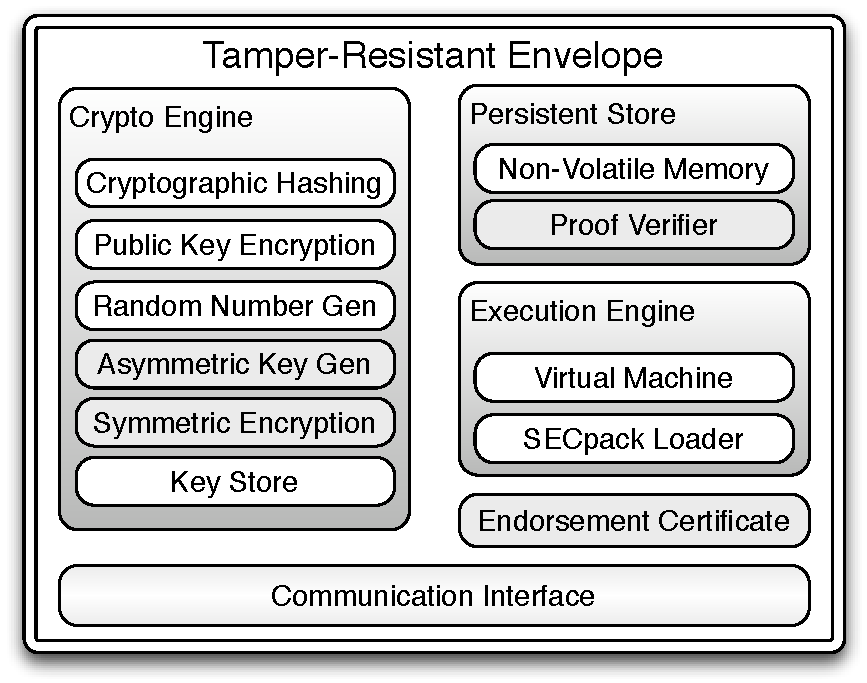
\includegraphics{omnifigs/tem_overview}
	}
	\caption{High-Level TEM Block Diagram}
	\label{fig:tem_overview}
\end{figure}

The TEM's cryptographic engine, covered in section \ref{arch:crypto}, is the
foundation of the TEM's security. The engine must provide random number
generation, cryptographic hashing\footnote{Cryptographic hashes are best
known in the context of digital signatures, where they are sometimes called
message digests.}, and asymmetric key encryption.

Section \ref{arch:execution} describes the TEM's execution engine, which
consists of a SECpack loader, and a stack-based virtual machine. The SEClosure code, local variables, and constant non-local variables are stored in the same flat addressing space. Encryption keys are stored by the cryptographic engine, and they are accessible via special-purpose instructions.

Mutable non-local variables are stored in the (intuitively named) persistent
store, whose design is covered in section \ref{arch:pstore}.

Aside from the main components described above, the TEM also contains a
communication interface, which is described in section \ref{arch:interface}.
The interface serves as an intermediary between the TEM's engines and the
outside world. The interface plays a distinct part when the communication
between the TEM and its owner occurs via untrusted channels, and needs to be secured.

The TEM must be accompanied by driver software which runs on the host computer.
For the sake of completeness, section \ref{arch:driver} summarizes the main
issues in the design of the driver software.

\section{Cryptographic Engine}\label{arch:crypto}

The design of the TEM's cryptographic engine has a huge impact on the TEM's
adoption rate. Cryptography algorithms account for most of the cost, die
size, and power consumption of a secure chip. Some cryptographic methods
carry legal implications, so the choices made here can place restrictions on
the TEM's adoption.

Furtermore, some algorithms incur a large computational effort, so incorporating
them has a severe impact on an application's response time. For example,
generating a 2048-bit RSA key takes a non-trivial amount of time, even on the
most powerful desktops available today. In order to alleviate this issue, the
functionality of the cryptographic engine is usually implemented in
hardware\footnote{Most chip vendors call it a cryptographic accelerator.}.

Fortunately, the Trusted Computing Group has already found good answers to
all of the concerns mentioned above, in their design of the Trusted Platform
Module (TPM) \cite{tcpa2007}. Therefore, the TEM's cryptographic engine
architecture builds heavily on the design of its counterpart in the TPM. This
section discusses the resulting design, and explains the significance of its
elements, in the context of the TEM.

\subsection{Random Number Generator}\label{arch:crypto_rng}
Genuine random numbers are needed as material for key generation, and to
implement nonces, which can be used to build freshness guarantees. Most secure
chips provide a true (hardware-based) random number generator, so this
requirement does not pose implementation issues.

\subsection{Cryptographic Hashes}\label{arch:crypto_hash}
The TEM's cryptographic engine must supply a cryptographically-strong hash.
The TEM needs this ability to verify the integrity of the information in
a bound SECpack, before executing the respective closure. Assuming the binding
process in section \ref{concepts:secpack_binding}, the cryptographic engine is
used to compute $h(\mathcal S || \mathcal P)$, so that it can be
compared with $\mathcal H$.

In order to meet or exceed the security guarantees provided by the TPM, the
cryptographic hash should be at least as strong as SHA1 \cite{eastlake2001rus}.
Fortunately, cryptography research has yielded good hash functions which are
in the public domain.

The TEM does not provide platform attestation to its host computer, so it does
not need to expose cryptographic hashing services directly.

\subsection{Asymmetric Key Cryptography}\label{arch:crypto_asymmetric}
Public key cryptography is the most heavyweight TEM component. It is necessary
because trusted execution requires a shared secret between the TEM and the
party that needs trusted execution guarantees, and secret distribution makes
symmetric encryption impractical.

Fortunately, the cryptographic accelerators on most secure chips provide
the basic asymmetric key operations, namely encryption, decryption, signing,
and signature verification. Also, the most common public encryption scheme,
RSA \cite{rivest1978mod}, has entered the public domain as of year 2000
\cite{rsasec2000}.

In order to be a secure alternative to the TPM, the TEM should support a
public-key encryption algorithm that yields at least the same security as
2048-bit RSA.

\subsubsection{Asymmetric Key Generation}
The only operation posing challenges is asymmetric key generation. In RSA, key
generation demands more resources than the other operations, by an order of
magnitude.

Key generation is not a hard requirement for a TEM. A manufacturer can choose
to generate the TEM's Private Endorsement Key outside the chip, at manufacturing
time, and then embed the key inside the TEM. The chain of trust in section
\ref{concepts:trust_chain} remains valid, as long as the manufacturer erases a
TEM's Private Endorsement Key from any medium outside that TEM, before the
TEM's Endorsement Certificate is generated.

If a TEM's cryptographic engine is incapable of asymmetric key
generation, TEM anonymity requires extra consideration. The process described
in \ref{concepts:anonymous_trust} can be modified to have the manufacturer's
server generate a User Key for the TEM. The manufacturer's server would then
give Mii the Private User Key (PrivUK) encrypted with the TEM's Public
Endorsement Key (PubEK).

There are secure chips capable of generating 2048-bit RSA keys, and they are
commercially available at reasonably low prices. Therefore, the rest of this
work will assume that the TEM's cryptographic engine provides asymmetric key
generation. It is straightforward to derive the architecture of a TEM without
such a generator, by removing the irrelevant features from the design presented
here.

\subsection{Symmetric Key Cryptography}\label{arch:symmetric_crypto}
Encryption algorithms that use private keys are a couple of orders of
magnitude faster than their public-key counterparts. This makes the
ability of performing symmetric encryption highly desirable.

However, symmetric key cryptography is heavily regulated by most legal systems.
For instance, the DES algorithm \cite{coppersmith1994} is still governed by
export restriction laws in the United States, at the time of this writing.
Furthermore, symmetric encryption is outlawed completetly in some countries. 

Making symmetric key cryptography a part of the TEM architecture would make the
platform vulnerable to legal issues, which would greatly hurt adoption. On the
other hand, private-key encryption cannot be ignored completely, due to the
performance advantages it provides. Therefore, the only logical step is to make
symmetric encryption an optional component of a TEM's cryptographic engine.

If a TEM chooses to offer symmetric encryption, the algorithm should provide at
least the same security guarantees as 128-bit AES \cite{daemen1999apr}. This is
necessary so that symmetric encryption does not become the weakest link in the
system. In other words, secrets protected by symmetric encryption should not be
easier to obtain than secrets protected by other means available in the TEM.

Symmetric cryptography is an optimization, and its presence or absence does
not significantly impact the overall TEM architecture.

\subsection{Secure Key Store}\label{arch:key_store}
A TEM cryptographic engine must provide secure key storage, and this
functionality is provided by the (again, intuitively named) key store. Figure
\ref{fig:key_store} provides a visual summary of the TEM's key store described
in this section.

\begin{figure}[hbtp]
	\center{
		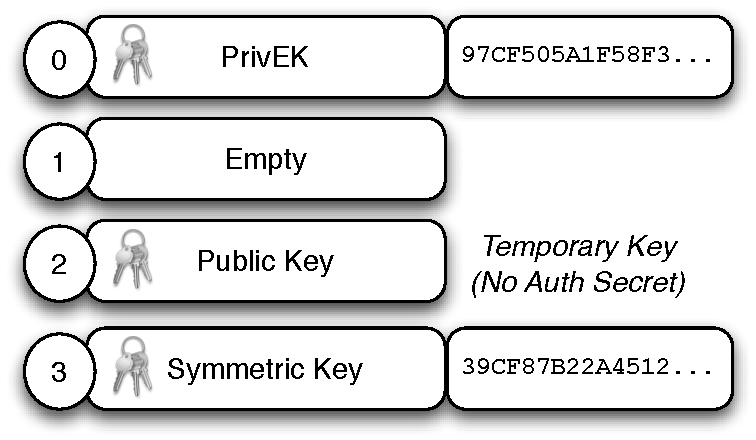
\includegraphics{omnifigs/key_store}
	}
	\caption{Snapshot of a TEM's Key Store}
	\label{fig:key_store}
\end{figure}

The key store is an array of key slots. A slot can store one of the following
encryption keys:
\begin{enumerate}
  \item the public component of an asymmetric key (also called a public key),
  \item the private component of an asymmetric key (also called a private key),
  or
  \item a symmetric key.
\end{enumerate}

The independent treatment of the two components of an asymmetric key is
insipired by the \texttt{javacardx.crypto} API in the JavaCard specification.
The advantage of this is that each key (corresponding to a slot) has
well-defined \texttt{encrypt} and \texttt{decrypt} methods, which would not be
true if both components of an asymmetric key would be amassed together in a
single slot.

A key created during SEClosure execution is temporary, which means it is released
when the closure which created it ends executing. A temporary key becomes
persistent when it is associated with an authorization secret. Authorization
secrets have the same size as a cryptographic hash (section
\ref{arch:crypto_hash}), and are used to regulate access to a TEM's persistent
keys. A closure is allowed to access a persistent key after presenting the
associated authorization secret.

An attractive aspect of this design is that no distinction needs to be made
for storing the TEM's Private Endorsement Key (PrivEK). PrivEK occupies the
first slot in a TEM's key store, and is associated with an authorization value
known only by the platform manufacturer. Furthermore, the manufacturer can
build ``privileged'' SEClosures, which use a TEM's PrivEK to offer additional
functionality. For example, TPM emulation, as well as the TEM anonymizing
scheme in section \ref{concepts:anonymous_trust} can be implemented as a
collection of ``privileged'' SEClosures.

\subsubsection{Considerations for Deleting Keys from the Store}
Allowing unauthorized key deletion does not compromise confidentiality, as no
information is disclosed. However, misuse of key deletion can lead to denial
of service attacks from misbehaving closures.

In order to prevent denial of service, a SEClosure is only allowed to delete from the key store the keys that it would be authorized to use as encryption / decryption keys.

On the other hand, a TEM owner must be allowed to delete persistent keys
from the store without having to know the authorization secret. Otherwise,
misbehaving closures may deny service to the TEM by filling up the key store.

\subsubsection{Motivation for the Key Store}
At a minimum, the cryptographic engine must be able to store the TEM's
Private Endorsement Key (section \ref{concepts:trust_chain}) for the TEM's
life. The engine must also be able to store one additional key, for the
duration of a closure's execution.

However, today's secure chips have enough resources to store many keys
simultaneously. This ability can be leveraged to reduce the number of times
that an often-used key must be loaded into the cryptographic engine. The
optimization can yield better execution times and smaller SECpacks, as a
SECpack does not need to contain a key that has already loaded into the TEM.
The cryptographic engine design cannot ignore these benefits.


\section{Persistent Store}\label{arch:pstore}
The persistent store is an associative memory backing the values of
mutable non-local variables for all the closures executing on the TEM. Section
\ref{concepts:pstore} argues that the most appropriate design is to identify
variables by addresses that are as large as cryptographic hashes, and use the
knowledge of a value's address as proof of authorization to access that
variable.

The conceptual presentation of the persistent store leaves out the following
issues:
\begin{itemize}
  \item the operations supported by the persistent store,
  \item the nature of the values in the store,
  \item the method for assigning an address to a variable, and
  \item bridging the gap between the possibility of executing a large number of
  SECpacks, and the small amount of non-volatile memory in the low-cost secure
  chips that the TEM targets.
\end{itemize}
The omission is deliberate, as the answers to these questions are engineering
trade-offs, and would have detracted from the understanding of the concept. This
section provides answers that are appropriate in the context of the TEM
architecture.

\subsection{Persistent Store Operations}
In the absence of a contrary reason, the persistent store provides the standard
associative memory operations:
\begin{itemize}
  \item \texttt{read(address)} returns the value stored at \texttt{address}, or
  a special \textsc{nothing} value if the persistent store does not have an
  association for the given address.
  \item \texttt{write(value, address)} writes \texttt{value} at
  \texttt{address}. \texttt{write} overwrites the old value stored at the given
  address, or creates a new association for \texttt{address}, and returns
  \textsc{created} or \textsc{updated} to reflect what happened. The return
  value is not relevant for a general understanding of the TEM archiecture, but
  it is needed in section \ref{arch:pstore_external}.
  \item \texttt{remove(address)} removes the value associated with
  \texttt{address}, if such an association existed.
\end{itemize}

\subsection{Persistent Store Values}
All the values in the TEM's persistent store are the size of the hashes
produced by the TEM's cryptographic engine (section \ref{arch:crypto_hash}).

Using fixed-size variables is essential to avoid complexity in the persistent
store implementation. Furthermore, an implementation that provides
variable-size values will end up using most (if not all) of the saved memory on
the bookkeeping required to make variable lookup fast.

The reasoning behind the chosen size requires some understanding of the TEM's
execution engine, described in section \ref{arch:execution}. The unique memory
space and the stack-based instruction set suggest a single attractive
alternative to the choices of value size: the size of a machine word. This
choice would make programming a bit more convenient, because it would be
possible to read a persistent store value directly onto the stack, or write
calculation results directly from the stack to the persistent store.

However, word-sized values  would cause memory waste, because a persistent
store value would be much smaller\footnote{The chips suitable for the TEM at
the time of this writing have a word size of 16 bits, whereas a SHA-1 hash
takes 160 bits.} than its address, so most of the memory would be spent on
addresses.

Furthermore, larger persistent store values can translate into speed benefits.
Closure compilers can bundle multiple variable values into the same persistent
store entry, in order to optimize speed. This will always yield benefits,
because reading/writing from/to the persistent store implies NVRAM, and
therefore is bound to be slower than multiplexing values in a closure's
RAM-backed memory space.

In conclusion, making persistent store values approximately the same size
as addresses makes sense for the TEM. The slight increase in complexity for the
closure compiler is rewarded by increased SECpack execution speed, and
better memory utilization.

\subsection{Persistent Store Address Allocation}\label{arch:ps_alloc}
The size of persistent store addresses must be at least as large as a symmetric
encryption key (section \ref{concepts:pstore}). This allows the following
allocation strategy: randomly choosing a persistent store address allocates that
address on all the TEMs in the world. Address allocation is used to mean that
no other closure will use the same address for a different variable. Address
allocation does not imply memory allocation on any TEM.

This strategy has the advantages that a variable has the same address on all
TEMs, and that address allocation can be done off-line. On the other hand, the
method's robustness is not immediately obvious, and guaranteeing integrity
against replay attacks is non-trivial. An argument for the method's robustness
is provided below. The discussion on preventing replay attacks is complex
enough that it has been assigned to its own section \ref{arch:pstore_freshness}.

\subsubsection{Robustness Argument}
Allocating an address uses the same mechanism as generating a symmetric
encryption key. Addresses are large enough that the chance of a conflict is not
bigger than the chance of generating an encryption key that belongs to someone
else. Most of the world's economy relies on symmetric encryption, as banks
communicate with each other using SSL \cite{freier1996ssl} or TLS
\cite{dierks1999tpv}, which in turn use symmetric encryption.

An argument similar to that in section \ref{concepts:pstore_auth} can be
used to show that the probability of having an attacker break the TEM trust
chain is much greater than the probability of having two SECpacks on the same
TEM that use the same address for different variables.

In closing it is worth noting that increasingly many systems rely on UUIDs
(Universally Unique Identifiers) \cite{leach2005ruu} for what is
essentially off-line address allocation. Using a hardware random number
generator to allocate a persistent store address is stronger than
the pseudo-random UUID allocation algorithm proposed in \cite{leach2005ruu}.
It is assumed that a SEClosure author has access to a good hardware RNG.

\subsection{Guaranteeing the Freshness in the Persistent
Store}\label{arch:pstore_freshness}
Guaranteeing freshness when the persistent store addresses are allocated 
offline requires some thought. It is non-trivial for a SEClosure to distinguish
between the case when its mutable non-local variables have never been used on a
TEM (and thus should be assumed to contain default values), and the case when
its variables have been assigned values, but the corresponding associations
have been \texttt{remove}d from the persistent store. The possibility of
confusing the two cases can be exploited by replay attacks.

\subsubsection{Preventing Replay Attacks: the Easy Way}
The straightforward method of eliminating the ambiguity is to specify
that once a persistent store association is created, it persists for the
lifetime of the TEM. In other words, the operation \texttt{remove} is forbidden.

When adopting this solution, the following concerns need to be addressed:
\begin{itemize}
  \item the persistent store grows proportionally to the number of
  non-local mutable variables used by SECpacks throughout the life of the TEM,
  and
  \item malicious SECpacks can initiate a denial of service attack by filling
  up the persistent store.
\end{itemize}

However, this solution is easier to understand and implement, so it may be more
desirable in some situations. All off the issues above can be worked around.

The persistent store entries can be stored in untrusted memory (as explained in
section \ref{arch:pstore_external}), and the capacities of both hard disks and
flash memories has been increasing at a rate that exceeds Moore's law. Denial of
service attacks can be prevented by placing a hard limit on the number of new
persistent store variables can be used by a SECpack.

\subsubsection{Preventing Replay Attacks: the Painful but Efficient Way}
The method of preventing replay attacks explained above is easy to understand,
but has a potential drawback in that all the non-local mutable variables
used on a TEM must persist forever, even if the SECpacks referencing them
will never be executed again. This section describes a more complex method for
preventing replay attacks that allows unused values to be \texttt{remove}d from
the TEM. The presentation requires a significantly deeper understanding of the
TEM as a whole, and is not as self-contained as the previous section.

The problem of preventing replay attacks can be reduced to avoiding the replay
of the initialization of the persistent store variables. This is because normal
SECpacks assume that the relevant mutable non-local variables have been
initialized prior to execution, so persistent store \texttt{read}s will never
return \textsc{nothing}. If this assumption is broken, a SECpack aborts its
execution and does not return any information  o the TEM owner. 

The only computation that is vulnerable to replay attacks is now the
initialization of persistent store variables. At-most-once semantics can be
provided for initializations by linking them to a monotonic counter inside the
TEM. This approach requires that a single value, the monotonic counter, has to
persis throughout the lifetime of the TEM. The rest of the section explains
the idea in more detail.

Let an \textbf{object}\footnote{Object-Oriented Programming is used to simplify
the presentation. However, the mechanism presented here can be easily
adapted to other programing paradigms.} be a group of SECpacks that use the
same mutable non-local variables. For convenience, an object's \textbf{fields}
shall be all the mutable non-local variables used by the SECpacks in the
object. Using the bank account example in section \ref{concepts:closures}, an
individual bank account is an object, and it consists of the SECpacks labeled
\texttt{withdraw}, \texttt{deposit}, \texttt{balance}, and \texttt{number}. The
bank account has one field, the variable \texttt{balance} (\texttt{number} is
optimized away by the closure compiler because it is de-facto immutable).

To reduce complexity, the lifetime of all the fields of an object are managed
at once, and management follows the same principles as constructors and
destructors (also named finalizers). Namely, an object is \textbf{constructed}
on a TEM by assigning initial values to all its fields. An object is
\textbf{destroyed} by \texttt{remove}-ing the values of its fields from the
persistent store. The SECpacks in an object will abort execution if any of
the fields they reference do not have a value in the persistent store,
because that means the TEM owner destroyed the object prematurely.

\subsubsection{Preventing Replay Attacks on Object Construction}
The solution is completed by ensuring that an object is constructed at most
once. A simple mechansim that achieves this goal is described below.

The mechanism uses a single monotonic counter, $\mathcal{M}_C$. The monotonic
counter's value is stored in the persistent store, at an address known only to
privileged SECpacks (described in section \ref{arch:key_store}). 

Constructing an object is achieved series of assignments to persistent store
addresses. The object's owner can construct a list of (address, value) tuples
that completely capture this information. This list is referred to as the
\textbf{constructor table}. 

Yu follows the following steps to produce an object that Mii can use on his
TEM:
\begin{enumerate}
	\item Mii runs a privileged SECpack that returns the value of
	$\mathcal{M}_C$, signed with the TEM's Private Endorsement Key, $r_v =
	\mathcal{M_C} || Enc_\textrm{PrivEK}(h(\mathcal{M}_C))$.
	\item Mii gives Yu $r_v$, the result of reading the
	counter, together with the TEM's Endorsement Certificate.
	\item Yu verifies ECert and the signature, to make sure that
	the Public Endorsement Key in the certificate can be trusted, and that
	the value of $\mathcal{M}_C$ is authentic.
	\item Yu binds the object's SECpacks to the TEM using PubEK,
	and also encrypts the \textbf{constructor data}, which is the constructor table
	together with the value of $\mathcal{M}_C$ that was verified in the previous step. The results produced
	at this step are given to Mii.
	\item Mii runs a privileged SECpack that decrypts the constructor data using
	PrivEK, and verifies that the value of $\mathcal{M}_C$ matches the value in
	the constructor data. If the verification is completed, then the SECpack
	carries out the \texttt{write}s described in the constructor table, and
	increments $\mathcal{M}_C$.
\end{enumerate}

It is easy to see that the process above does not allow an object
to be constructed twice -- exactly one object is constructed for a certain
value of $\mathcal{M}_C$. Guaranteeing that Mii cannot replay the constructor
assignments translates into guaranteeing freshness for the fields of an
object, which are, by definition, all the values that SECpacks will read
from the persistent store.

\subsection{Secure External Memory: The World in a
Nutshell}\label{arch:pstore_external}
Section \ref{concepts:pstore} explains that the persistent store must protect
its contents from attempts of bypassing the associative memory interface.
This leads to the straightforward implementation of storing all the
associations in non-volatile memory shielded by the TEM's tamper-resistant
envelope. Unfortunately, secure NVRAM is expensive, so it does not come in
abundance on the low-cost chips that the TEM targets. This section analyzes the
possibility of using untrusted memory outside the TEM's secure envelope, which
is significantly less expensive.

The TEM uses the approach to external secure memory introduced by the AEGIS
\cite{suh2003aat} secure processor, which leverages Merkle trees
\cite{merkle1980ppk}. The persistent store's external memory design adapts the
maintainance algorithms to the TEM scenario (a low-cost chip attached to a
powerful, but untrusted processor), and modifies the design slightly to obtain a
hash tree whose height is logarithmically proportional to the number of
associations inside the TEM, and not to the size of the addressing space.

Like AEGIS \cite{suh2003aat}, the persistent store relies on building a tree,
where the leaves store the actual associations, and internal nodes store a
cryptographic hash of their children\footnote{Optimized designs that allow
internal nodes to store associations together with the hash of their children are
reasonably straightforward.}. The tree's root must be stored in NVRAM inside the
TEM's secure envelope, but all the other nodes can be stored in untrusted memory.

In order to ensure the integrity and confidentiality of the data, neither the
persistent store addresses nor the values can be stored ``in the clear'' in
untrusted memory. A symmetric encryption key\footnote{The symmetric
key never leaves the TEM, and can be generated cheaply using a PUF
\cite{gassend2002spr}. }\footnote{If the law does not allow symmetric encryption, an asymmetric key is used instead. Note that the persistent store becomes painfully inefficient in this case.} that is also stored inside the TEM's NVRAM is used to encrypt the associations. The
two parts of an association must be encrypted individually, so that the TEM can
later ask for an association by its encrypted address. This external
representation is used for computing the hashes in the internal nodes, so the
contents of the internal nodes are not confidential.

The TEM's host (with a powerful but untrusted processor) is responsible for
maintaining the tree structure. When a persistent store \texttt{read} is
issued, the TEM communicates the encrypted persistent store address to the
host. The host responds with the encrypted value associated with the
address, together with a proof of correctness consisting of the contents of all
the intermediary nodes. A \texttt{write} is handled similarly, except that the
correctness proof also describes the updates that must be performed to the
tree.

\subsubsection{Amnesia and Replay Attacks}
The tree used for external memory storage is said to exhibit
\textbf{amnesia} if it is possible for the TEM's host, who is managing the tree,
to ``forget'' about a persistent store association. The host would tell the
TEM that an entry does not exist, when in fact it does. Assuming the persistent
store implementation mistakenly believes the owner, the net result would be
that a \texttt{read} could return \textsc{nothing} when it should return a
value, and a \texttt{write} could return \textsc{created} instead of
\textsc{updated}.

An external memory tree exhibiting amnesia is \textbf{acceptable} if the
persistent store design, as a whole, can be used to detect the wrong answers
that can be originated by amnesia and report that the external tree has been
compromised.

Amnesia is important for the persistent store design. External
memory trees that are guaranteed to either provide the correct answer or
exhibit amnesia have a much simpler structure than trees that must provde the
correct answer, without the possibility of amnesia. If amnesia is not
acceptable, then the external tree sturcture must allow the TEM's host to
construct a prof that a tree contains no association for a given address. On
the other hand, if amnesia is allowed, then the host computer can structure the
tree as it wishes, and it does not need to provide a proof when claiming that
the tree does not contain any association for a certain address.

A necessary, but not sufficient, condition for amnesia to be acceptable is that
the correct return value of a \texttt{write} (\textsc{created} or
\textsc{updated}) is known in advance. In other words, whenever a variable is
assigned a value, the persistent store should know whether the store already
contains a corresponding association or not. Otherwise, the host can trick the
TEM into creating two leaves for the same association, and later lead the TEM
to the leaf corresponding to a stale value.

The method of guaranteeing persistent store freshness (section
\ref{arch:pstore_freshness}) determines if amnesia is acceptable. For example,
the straigthforward method described at the beginning of section
\ref{arch:pstore_freshness} requires the guarantee that the persistent store
will not exhibit amnesia, because its correctness relies on receiving the
correct answer from \texttt{read}, and amnesia means that a \texttt{read} may
return \textsc{nothing} when it shouldn't.

On the other hand, the more complicated method described in the same section
works correctly even when faced with amnesia, because it must work correctly
even when the TEM owner \texttt{remove}s associations (intuitively, amnesia
resembles spurious \texttt{remove}s.) The complicated method works correctly
becauseit is known that all the SECpacks of an object will issue only
\texttt{writes}s that return \textsc{updated}, and only \texttt{reads} that do
not return \textsc{nothing}. Also, all the \texttt{write}s in a constructor
are guaranteed to return \textsc{created} under normal use, but this condition
does not need to be verified to insure the correctness of the persistent store
operations.

\subsubsection{Preventing Amnesia}
If the persistent store is not allowed to exhibit amnesia, the host must be
able to prove that an association does not exist in the tree. In order for the
proof to have an efficient encoding (i.e., not enumerate all the leaves in the
tree), there must be a single possible path from the root to a leaf containing
a certain address.

The fixed tree in AEGIS \cite{suh2003aat} trivially meets the requirement
above, but is not ideally suited for a sparse addressing space, because its
height is proportional to the number of bits in an address. The issue is
exacerbated by the pressure of the low-memory TEM environment on the
tree's branching factor. For example, assuming SHA1 is used for
hashing, a branching factor of 1,000 would require 20KB of RAM for storing a
single internal node. 20KB is a luxury in the low-cost chips that the TEM is
targeting. On the other hand, using a really small branching factor increases
the tree depth and lowers performance.

A binary search tree is an attractive alternative, especially because the tree
\emph{does not have to be balanced}. Intuitively, it is safe to assume that the
tree will perform according to the average-case analysis, because the tree keys
are encrypted addresses, so they will ``look'' random. Formally, a misbehaving
SEClosure cannot cause the persistent store to produce a worst-case tree structure, because it cannot guess the addresses that would encrypt to keys that would lead to the worst-case tree structures.

Implementing the binary search trees requires that internal nodes would have to
be augmented to also store addresses, which is straightforward. An optimized
implementation will tweak the tree's branching factor to achieve a good
compromise between the size of an internal node and the tree's height.

\section{Execution Engine}\label{arch:execution}
The execution engine processes SECpacks synchronously, according to
the following simple loop:
\begin{enumerate}
  \item load a SECpack provided by the communication interface,
  \item carry out the computation expressed in the SECpack,
  \item provide the computation result to the communication interface, and
  \item release resources and prepare for the next SECpack.
\end{enumerate}

\subsection{The TEM Virtual Machine}\label{arch:vm}
The computation inside a SECpack is expressed as microinstructions
for a stack-based virtual machine (VM). The virtual machine stores code and data
in a single, flat memory space (described in detail later). The entire VM
interpreter state consists of the following registers:
\begin{enumerate}
  \item {IP (the instruction pointer)} is the memory address of the instruction
  that will be executed next, and
  \item {SP (the stack pointer)} is the memory
  address of the top of the VM's stack.
\end{enumerate}

Instructions are encoded as a 1-byte operation code (opcode), optionally
followed by immediate data. The size of the immediate data following an opcode
can be determined by looking at the opcode, to make code analysis easy.

The stack has a conventional design: it consists of fixed-size entries, which
are the size of the machine word. Unless otherwise specified, instructions read
their inputs by popping entries off the stack, and push their results onto the
stack.

\subsubsection{Standard Operations}
The virtual machine has standard instructions for performing arithmetic
operation, stack manipulation, and execution flow control.

\subsubsection{Single Memory Space}
The TEM's execution environment provides a single RAM-backed memory space that
contains the closure's executable instructions, values of local variables and de-facto
immutable non-local variables, and the virtual machine's stack.

Although the TEM's VM has a stack-based instruction set, closures have
unrestricted access to the memory space. This offers maximum flexibility (e.g.,
self-modifying code) that closure compilers can use to squeeze one last drop
of performance out of the execution engine.

\subsubsection{The Output Buffer}
The output buffer is an append-only memory zone, and its role is to make
building secure closures easier. If a closure terminates successfully by
executing \texttt{halt}, the contents of the output buffer is returned as the
result of the execution. In case an exception occurs during execution, nothing
is returned. Therefore, the output buffer is intended to help developers build
secure closures, by demanding that they make an active effort to report a piece
of data as a result.

\subsubsection{Persistent Storage Interface}
The contents of mutable non-local variables is stored in the TEM's persistent
store (sections \ref{concepts:pstore} and \ref{arch:pstore}) between
executions. Addresses are stored in memory space, and values are transferred
between the memory space and the persistent store. The instructions for working
with the persistent store closely mirror the interface presented in
section \ref{arch:pstore}.

\subsubsection{Cryptographic Engine Interface}
The execution engine offers interfaces to all the functions of the
cryptographic accelerator described in section \ref{arch:crypto}.

A closure is automatically authorized to use all the encryption keys that it
creates. The SEClosure can use keys that are already loaded in the cryptographic
engine, once it demonstrates knowledge of their authorization secret. The
execution engine enforces these restrictions by keeping track of the keys that
the closure is authorized to use. If a closure attempts to use a key before
gaining authorization, its execution is aborted. The execution engine
also keeps a list of the temporary keys produced by a SEClosure, and removes them at the end of the closure's execution.

Keys in the cryptographic engine's store are identified by the number of the
slot storing them. Unless otherwise specified, the cryptographic instructions
read/write key identifiers from/to the VM stack.

\subsection{Design Philosophy}\label{arch:vm_philosophy}
This section describes the issues encountered in the design the TEM's
execution engine, and explains the reasoning behind the trade-offs that were
made.

\subsubsection{Motivation for Synchronous Execution}
The execution engine design completely discards any possibility of concurrent
execution. The factors driving this decision are:
\begin{itemize}
  \item Concurrent programming is notoriously hard to get right, so
  applications demanding provable security tend to forgo the speed benefit
  anyway.
  \item At the time of this writing, all existing low-cost secure chips contain
  a single general-purpose execution core, so provisions for concurrent
  executions would not be readily applicable.
  \item A multi-core TEM can be modeled as multiple execution engines that
  share a persistent store. The consistency of the persistent store is ensured 
  by treating each SECpack execution as a transaction. This design is much
  easier to implement correctly, as it relies on heavily-studied techniques
  from the database world.
\end{itemize}

\subsubsection{Motivation for the Single Memory Space}
The clear separation between the RAM-backed memory space and the consistent
store provides optimum performance in low-resource environments. Most
operations reference RAM memory, which yields speed and increases EEPROM
lifetime.

Since the single memory space contains a closure's code, allowing unrestricted
access to that memory space makes static verification techniques (used in the
Java Virtual Machine) impossible to apply. This is not an issue for the TEM, as
the target hardware does not have the resources needed for static verification,
so dynamic verification is unaviodable.

The TEM would not benefit from a more complex memory scheme. Segmented memory
would not be useful, since the execution engine is synchronous, so code sharing
cannot occur. Paged memory is also not interesting, because the TEM does not
have multiple code privilege levels, or virtual memory.

\subsubsection{Motivation for a Virtual Machine}\label{arch:vm_motivation}
Using a virtual machine carries a price in performance, but makes the the executable code in a SECpack universal. Having SECpack executable code
target specific hardware introduces complexity (multiple target platforms) for
the closure compiler, and blocks SECpacks from being migrated among TEMs.

The TEM's virtual machine plays a bigger role in execution speed than commodity
VMs that are targeted towards desktop computers (e.g., the Java Virtual Machine
\cite{lindholm1999jvm}, and ECMA Common Intermediate Language
\cite{standard2001cli}) because the TEM is not powerful enough to perform
Just-In-Time Compilation (JIT). Thus, on the TEM, even performance-critical
code is running under the VM interpreter, whereas desktop virtual machines
can translate ``hot'' code to the hardware's native instruction set.

On the other hand, the performance degradation introduced by the virtual machine
has no significant impact on most TEM applications. Assuming a reasonable VM
implementation, a single asymmetric key encryption operation dwarfs the cost of
interpreting thousands of VM instructions. Public-key encryption is invoked
for every bound SECpack, because a part of the SECpack must be decrypted with
the TEM's Private Endorsement Key.

\subsubsection{Motivation for a Stack-Based Instruction
Set}\label{arch:stack_motivation}
Having established that the TEM will use a virtual machine makes the
decision of using a stack-based instruction set relatively straight-forward.

Stack-based instruction sets are easy to generate from ASTs (Abstract Syntax
Trees), and are a decent intermediate representation for code analysis
algorithms. Stack-based instruction sets also yield the smallest possible code.
If JIT (Just-in Time Compiling) becomes a possibility, simple register
allocators can turn stack-based code into native code with very good
performance. 

Using a register-based instruction set doesn't make much sense for an
interpreted virtual machine. The real processor registers are likely to be used
up by the VM interpreter, so virtual registers would end up being simulated by
RAM, which results in the same speeds seen by stack-based languages, at the
cost of a more complex implementation.

Stack-based instruction sets are used in recent VMs for both medium-level
languages (e.g., the Java Virtual Machine \cite{lindholm1999jvm}) and high-level
languages (the Ruby 1.9 VM \cite{sasada2005yya}).

\subsubsection{Considerations in the Design of the Instruction
Set}\label{arch:vm_instructions}
The standard instructions are heavily inspired by the Java Virtual Machine
\cite{lindholm1999jvm}. The TEM-specific instructions (cryptography and
persistent store) have been developed trying to apply the same principles.

The instruction set tries to strike a balance between enabling small SECpacks
and keeping the VM interpreter simple. For example, most instructions operating
on memory blocks have two variants. The fixed block variant (instructions ending
in \texttt{fxb}) receives the information about the blocks (address, and
optionally length) as immediate data, which optimizes SECpack size. The
variable block variant (instructions ending in \texttt{vb}) pops the block
information off the stack, for maximum efficiency when working with
variable-length memory structures. Exceptions were made for instructions that
would not occur often in a SECpack (e.g., \texttt{rnd}), so the space savings
do not warrant the extra complexity in the interpreter.

The design of the TEM-specific instructions was biased by my laziness which
pushed me to keep the prototype implementation simple.

The instruction set aims for consistency with respect to mnemonics and
order of parameters. A few examples:
\begin{itemize}
  \item \texttt{ld} (load) instructions push data on the stack, and \texttt{st}
  (store) instructions write data to the memory space,
  \item \texttt{fxb} (fixed-block) instructions receive their parameters in the
  same order that they should be pushed on the stack for the corresponding
  \texttt{vb} (variable-block) instructions, and
  \item instructions that receive the same parameters (e.g., \texttt{mcfxb} and
  \texttt{mcpyfxb}) have the same parameter order.
\end{itemize}
Aside from making the VM easier to understand, consistency can be leveraged
to optimize the interpreter code.

\subsection{The SECpack Loader}\label{arch:secpack_loader}
A SECpack consists of a snapshot of the initial state of the virtual machine's
memory space, together with a header containing a magic value, the initial
values for the VM's instruction pointer and stack pointer, and data needed to
decrypt a bound SECpack. This makes virtual machine setup trivial, given an
unbound SECpack.

A bound SECpack (section \ref{concepts:secpack_binding}) requires that the
loader decrypts the private information $\mathcal{P}$ and verifies the
integrity of the shared information $\mathcal{S}$. The process for doing this
is straightforward, and implies reversing the steps of the binding process
described in section \ref{concepts:secpack_binding}. The SECpack header
contains the sizes of the $\mathcal{S}$ and $\mathcal{P}$ areas, and an unbound
SECpack is indicated by an empty $\mathcal{P}$ area.

When the SECpack loader is invoked, it is given the SECpack and the number of
a slot in the cryptographic engine's key store. The key in that slot is used to
decrypt the SECpack. The loader must reject bound SECpacks that fail the
integrity check $\mathcal{H} = h(\mathcal{S} || \mathcal{P})$.

The ability of using arbitrary keys (as opposed to PrivEK alone) for decrypting
SECpacks allows for speed optimizations and extensions to the TEM's chain of
trust. For example, an often-used set of SECpacks can be bound to a TEM using a
symmetric key instead of PubEK, if the key is transmitted securely to the
TEM by encrypting it with PubEK. This can significantly decrease execution time
by avoiding an asymmetric-key decryption operation every time the SECpacks are
loaded.

The TEM trust chain is not compromised by allowing arbitrary keys to be
used as SECpack decryption keys, because of the integrity check that occurs after
SECpack decryption, and because of the magic value in the header. 

\subsection{The TEM Instruction Set}
For the sake of completeness, this section briefly describes the instructions
that make up the VM Instruction Set. Although the instruction set is usually
considered an implementation detail, the VM's instruction set is necessarily a
part of the TEM's architecture. All TEMs, regardless of the hardware
implementation, will have to implement the same instruction set. The
instruction set presented here is not completely optimized, but it is a good
starting point, as it is working well in the prototype TEM implementation. 

The instructions are a straightforward application of the design principles set
forth in section \ref{arch:vm_philosophy}, combined with bits shamelessly
stolen from the other architectures I have worked with. Most readers can safely
skip this section.

\subsubsection{Standard Operations}
The standard instructions, classified by their purpose, are:
\begin{itemize}
  \item arithmetic operations; \texttt{add}, \texttt{sub} (subtract),
  \texttt{mul} (multiply), \texttt{div} (division quotient), \texttt{mod}
  (division reminder) perform respective arithmetic operation on the top two
  numbers in the stack, and push the result on the stack.
  \item flow control; \texttt{halt} marks the successful completion of a
  closure's execution. \texttt{jmp} changes the value of the IP register
  (``jumps'') unconditionally, as opposed to the conditional jump instructions that only change IP if the value at the top of the stack meets the condition in the instruction name. The conditional jumps are (unsurprisingly) \texttt{jz} (jump if zero), \texttt{jnz} (jump if not zero),
  \texttt{ja} (jump if above zero), \texttt{jb} (jump if below zero),
  \texttt{jae} (jump if above or equal to zero), and \texttt{jbe} (jump if
  below or equal to zero). The new IP value is encoded as immediate data for
  each of the flow control instructions.
  \item stack manipulation; \texttt{ldbc} (sign-extend and load/push a 1-byte
  constant), \texttt{ldwc} (load/push a 1-word constant), \texttt{pop} (pop one
  item), \texttt{popn} (pop $N$ items), \texttt{dupn} (duplicate the top $N$
  items), \texttt{flipn} (reverse the order of the top $N$ items) are rather
  straightforward. Constants are encoded as immediate data. $N$ is considered a
  constant encoded as 1-byte unsigned number.
\end{itemize}

\subsubsection{Single Memory Space}
The following instructions for interfacing with the memory space take one
immediate value, which is the address that they read from / write to.
\begin{itemize}
  \item \texttt{ldb} (load byte): sign-extends and loads/pushes a byte in the
  memory space
  \item \texttt{ldw} (load word): loads/pushes a word beginning at the
  given address in the memory space
  \item \texttt{stb} (store byte): pops the top word off the stack and stores 
  its least-significant byte in the memory space
  \item \texttt{stw} (store word): pops the top word off the stack and stores
  it beginning at the given address in the memory space
  \item \texttt{mcfxb} (memory-copy, fixed block): copies a memory block
  (contiguous sequence of bytes) to another memory location; the operation
  parameters (address and length of the source block, address where the block
  will be copied) are encoded as word-sized immediate values
  \item \texttt{mcvb} (memory-copy, variable block): analogous to
  \texttt{mcfxb} that pops the operation parameters off the stack
  \item \texttt{mcmpfxb}, \texttt{mcmpvb} (memory-compare, fixed /
  variable blocks): lexicographically compare the contents of two memory blocks
  and store the comparison result on the stack; the buffers are identified
  using the same parameters as in \texttt{mcfxb}, and respectively \texttt{mcvb}
\end{itemize}

The instructions \texttt{ldbv} (load byte from variable address), \texttt{ldwv}
(load word from variable address), \texttt{stbv} (store byte at variable
address), and \texttt{stwv} (store word at variable address) behave similarly
to the instructions explained above, but they use the stack to read the
memory address that they will operate on. These instructions are useful when
dealing with variable-size data structures.

\subsubsection{The Output Buffer}
The instructions interfacing with the output buffer are:
\begin{itemize}
  \item \texttt{outnew} (new output buffer): creates the output buffer for a
  SEC; reads the word from the top of the stack as an upper limit of the number
  of bytes that will be written to the output buffer (an exception will be
  generated if the SEC exceeds the limit)
  \item \texttt{outb}, \texttt {outw} (output byte / word): same behavior as
  \texttt{stb}, \texttt{stw} except they target the output buffer
  \item \texttt{outfxb}, \texttt{outvb} (output fixed / variable block): same
  behavior as \texttt{mcfxb}, \texttt{mcvb}, except the destination is the
  output buffer
  \item \texttt{outvlb} (output variable-length block): a compromise between
  \texttt{outfxb} and \texttt{outvb} -- the address of the source memory buffer
  is fixed (encoded as immediate data), but the length is obtained from the
  stack
\end{itemize}

As a further optimization on SECpack size, a destination address equal to the
maximum word size (i.e., \texttt{0xFFFF} on 16-bit processors) is interpreted
as ``the destination is the output buffer''.

\subsubsection{Persistent Storage Interface}
The instructions for interfacing with the persistent store are:
\begin{itemize}
  \item \texttt{pswrfxb}, \texttt{pswrvb} (persistent store write using
  fixed/variable blocks): write a value from the memory space into the
  persistent store. Their parameters are the addresses of the memory blocks 
  containing the persistent store address and the value to be written. The
  instructions map to the \texttt{write} method presented in \ref{arch:pstore}.
  \texttt{pswrvb} has variable parameters (coming from the stack), whereas
  \texttt{pswrfxb} uses fixed parameters (encoded as immediate values).
  \item \texttt{psupfxb}, \texttt{psupvb} (persistent store update using
  fixed/variable blocks): similar to \texttt{pswrfxb}, \texttt{pswrvb}, but abort
  execution if the persistent store had no association for the given address (the
  underlying \texttt{write} would have returned \textsc{created})
  \item \texttt{psrdfxb}, \texttt{psrdvb} (persistent store read using
  fixed/variable blocks): read a value from the persistent store into the
  memory space. The parameters mirror \texttt{pswrfxb}, and respectively
  \texttt{pswrvb}. An execution is generated if the persistent store does not
  have a value associated with the given address.
  \item \texttt{pshk} (persistent store has key): looks up an address in the
  persistent store. The persistent store address is stored in a variable block
  (its location in memory space is read from the stack). The result is
  \texttt{1} if the persistent store contains an association for the given
  address, and \texttt{0} otherwise. The result is pushed on the stack.
  \item \texttt{psrm} (persistent store remove): removes a value from
  the persistent store, using the semantics of \texttt{remove} in
  \ref{arch:pstore}. The only parameter is the address of memory block
  containing the peristent store address. The parameter is read from the stack.
\end{itemize}

\subsubsection{Cryptographic Engine Interface}
The following instructions manage the encryption keys for the algorithms 
covered in sections \ref{arch:crypto_asymmetric} and
\ref{arch:symmetric_crypto}:
\begin{itemize}
  \item \texttt{genk} (generate key): generates a symmetric or asymmetric
  encryption key. The desired key type is encoded as a 1-byte immediate value.
  Upon successful completion, the instruction will push on the stack the
  slot/slots holding the generated key (an asymmetric key requires two slots).
  \item \texttt{relk} (release key): unloades a key from the crypto store.
  \item \texttt{ldkl} (load key length): pushes on the stack an upper bound for
  the length (in bytes) required to hold the serialized version (via
  \texttt{stk}) of a key.
  \item \texttt{rdk} (read key): creates a crypto store key by reading
  a serialized version (via \texttt{stk}) of the key from a memory block. The
  address of the memory block is popped from the stack. Upon success, pushes the
  number of the slot holding the new key on the stack.
  \item \texttt{stk} (store key): writes a serialized version of a key into the
  memory space. The address of the memory block and the slot number are read
  from the stack.
  \item \texttt{authk} (authorize key): pops off the stack a slot number and
  the address of a memory block containing an authorization secret. If the slot
  contains a temporary key, it is made persistent by attaching the authorization
  secret. Otherwise, the authorization secret is presented to gain access to
  the key. An execution exception occurs if the presented secret does not match
  the authorization secret associated with the key.
\end{itemize}

The encryption keys can be used to:
\begin{itemize}
  \item encrypt and decrypt data, via \texttt{kefxb}, \texttt{kevb},
  \texttt{kdfxb} and \texttt{kdvb} (keyed encrypt/decrypt using fixed/variable
  memory blocks), and
  \item produce and verify signatures, via \texttt{ksfxb}, \texttt{ksvb},
  \texttt{kvsfxb} and \texttt{kvsvb} (keyed sign/verify signature using
  fixed/variable memory blocks).     
\end{itemize}
The instructions above take the following parameters: the slot number of the
key to be used (always read from the stack), the address and length of the
block of data to be used as input, and the address where the output shall be
written. The last three parameters can be fixed (encoded as immediate values) or
variable (read from the stack).

The hashing function (section \ref{arch:crypto_hash}) in the cryptographic
engine is accessed by the instructions \texttt{mdfxb}, and \texttt{mdvb}
(message-digest using fixed/variable blocks). The instructions resemble those
for copying memory blocks (\texttt{mcpyfxb}, and \texttt{mcpyvb}) but, instead
of writing a copy of the source block, they write a cryptographic hash (also
known as a message digest) of the source block.

The random number generator (section \ref{arch:crypto_rng}) is invoked by the
instruction \texttt{rnd} (random), which writes random data to the memory
space. \texttt{rnd}'s two parameters are read from the stack, and they indicate
the desired number of random bytes, and the memory address where the random
bytes will be written.

Encryption keys are stored by the cryptographic engine. A closure's memory
space may contain serialized encryption keys, but these keys have to be loaded
into the cryptographic engine before they can be used in cryptographic
operations. If a TEM can generate encryption keys, the VM provides instructions
for serializing the keys into the running closure's memory space. 

\section{Communication Interface}\label{arch:interface}
The main component of the TEM's communication interface is a transceiver for
the communication channel between the TEM and its owner. This channel can be an
external bus such as the Universal Serial Bus \cite{specification2000r} if
the TEM is a physically distinct computer add-on, or an internal bus such as
the PCI local bus \cite{specification1998r} or the LPC (low pin-count) bus
\cite{intel2002lpc}, if the TEM is included on the system's motherboard.

If the communication channel between the TEM and its owner is insecure, the
communication interface abstracts this problem away from the rest of the TEM
modules, by establishing a secure session. The mechanism for establishing the
secure session is inspired by SSL \cite{freier1996ssl}, but simplified by the
lack of protocol negotiation. A rough outline of the required steps is:
\begin{enumerate}
  \item the TEM sends its Endorsement Certificate,
  \item the owner validates the Endorsement Certificate and is assured that the
  Public Endorsement Key (PubEK) belongs to a TEM,
  \item the owner generates a symmetric encryption key\footnote{if the laws prohibit symmetric
  encryption, an asymmetric encryption key can be used instead} to be used as a
  session key,
  \item the owner encrypts the session key with the TEM's PubEK and sends it to
  the TEM,
  \item the TEM uses its Private Endorsement Key (PrivEK) to decrypt the
  session key, and
  \item the TEM and the owner use the session key to communicate securely.
\end{enumerate}


\section{Driver Software for the TEM Host}\label{impl:driver}
The prototype implementation of the TEM's driver is not at all what one would
expect to find in a driver. The low-level details of communicating with the
TEM smart card are handled by the \textsc{smartcard} Ruby extension described
in section \ref{impl:rubygem}. Ruby makes encoding and decoding APDUs trivial,
as demonstrated by listing \ref{impl:driver_alloc_buffer}, which contains the
code for allocating a buffer on the TEM. This left time and energy for higher
level features that are rarely present in production drivers, let alone
research prototypes.

\lstinputlisting[float=bph, language=Ruby, caption=TEM Buffer Allocation
Implementation in the Ruby Driver,
label=impl:driver_alloc_buffer]{code/drv_alloc_buffer.rb}

\subsection{Domain Specific Languages}
Ruby is a highly dynamic language, and it is very suited for producing DSLs
(domain-specific languages), as demonstrated in \cite{cuadrado2007bds} and
\cite{cunningham2007rmr}. DSLs are part of the ``magic'' that is responsible
for the huge success of the Ruby on Rails \cite{thomas2006awd} framework. The
TEM driver uses two DSLs directly. A small language describes the primitive
data types on a TEM, and a second-order DSL\footnote{(a DSL that generates
another DSL)} expresses all the necessary information for assembling SEClosures.

The primitive data types DSL takes types one-line type definitions and
produces functions necessary for encoding and decoding numbers corresponding to
these data types. For instance, the definition for \texttt{byte} at the
beginning of listing \ref{impl:driver_types_dsl} yields the methods
\texttt{read\_tem\_byte}, \texttt{to\_tem\_byte}, and
\texttt{tem\_byte\_length}.

\lstinputlisting[float, language=Ruby, caption=TEM Primitive Data Types
Expressed using the DSL, label=impl:driver_types_dsl]{code/drv_types_dsl.rb}

The DSL describing the instruction set of the TEM is a second-order DSL. The
instruction set DSL, illustrated in listing \ref{impl:driver_instructions_dsl},
constitutes the backbone of the TEM assembler. An instruction definition in the
DSL contains user-friendly names for the instruction and its parameters, as
well as precise instructions on how to encode the instruction for the TEM's VM.

\lstinputlisting[float, language=Ruby, caption=Memory Block Instructions
Expressed using the DSL,
label=impl:driver_instructions_dsl]{code/drv_instructions_dsl.rb}

The Ruby driver features a state of the art SECpack assembler that supports
commens, multiple instructions per line, named parameters, named labels,
human-readable immediates, macros written in Ruby, and line-level debugging
information (exploited for the advanced developer support described  in section
\ref{impl:driver_dev_support}). Relating to the bank account example introduced
in section \ref{concepts:closures}, listing \ref{impl:driver_balance_secpack}
shows a possibile implementation of the \texttt{balance} SEClosure. The power of
the assembly language is illustrated well by the SECpack source in listing
\ref{impl:driver_keygen_secpack}. Most features were obtained at very little
cost, by using a DSL to represent the assembly language. This DSL is generated
from the instruction set DSL described above.

\lstinputlisting[float=hbt, language=Ruby,
caption=Assembly code for \texttt{balance} in the bank account example,
label=impl:driver_balance_secpack]{code/drv_balance_secpack.rb}

\lstinputlisting[float=hbt, language=Ruby, caption=Assembly Code for
Key-Generating SECpack, label=impl:driver_keygen_secpack]{code/drv_keygen_secpack.rb}

The set of DSLs presented here made experimenting fun again. Once the code for
interpreting the DSLs was solid, and the initial definitions were created, it
became really easy to change the definitions to experiment variations in
encoding data types or instructions. Because the DSLs are so easy to maintain,
they have become the authoritative specifications for the TEM's encoding
mechanisms.

\subsection{Developer Support}\label{impl:driver_dev_support}
The powerful assembly language described above plays a major role in making it
easy to develop SEClosures for the TEM. The other two big features are a full
suite of unit tests, and meaningful translations for SEClosure execution errors.

The TEM driver contains a full\footnote{\texttt{rcov} indicates a line coverage
of 95\% or above on each Ruby source file.} suite of unit tests, covering both
driver and firmware code. The unit tests have proven to be a very good
investment, as they have automated the following tasks:
\begin{itemize}
  \item validating the Ruby driver implementation,
  \item validating any TEM firmware implementation, 
  \item assessing the suitability of a JavaCard model as a TEM, and
  \item assessing the compatibility of a smart card reader with the TEM driver
  stack.
\end{itemize}

When any of the layers above exhibits a bug, a failing unit test provides a good
starting point for investigation. However, if the failure is a SEClosure execution exception, the Ruby driver goes one step further, by retrieving the TEM's execution engine status (using the features in section
\ref{impl:fw_dev_support}), and combining it with line-level debugging
information. The result is the ability to pinpoint the exact SECpack
instruction that caused the failure. Listing \ref{impl:driver_exception} shows
the data obtained from a typical SEClosure execution exception. Quick inspection
reveals that the exception occured during the \texttt{outw} instruction, and the
instruction was assembled in file \texttt{test\_exceptions.rb} at line 32. The
information includes a snapshot of the execution environment at the time of the
exception.

\lstinputlisting[float, language=Ruby, caption=Debugging Information for a SEClosure Execution Exception, label=impl:driver_exception]{code/drv_exception.txt}

This level of support is hard to find in research prototypes. It is present in
the TEM's driver because Ruby's dynamic features drove the cost of implementing
the features below the time that they saved.

\chapter{Prototype Implementation}\label{impl}
The Trusted Execution Module is not just a collection of abstract ideas. I have
implemented the complete TEM architecture described in chapter \ref{arch} in a
thumb-sized tamper-resistant chip that can be mass-produced at a unit cost of
less than 5 USD.

The prototype implementation served as a platform for experimentation
throughout the TEM's development, and provides concrete proof that the
proposed TEM design is practical.

The prototype TEM implementation consists of the following software modules:
\begin{itemize}
  \item The TEM architecure described in chapter \ref{arch} is implemented by
  the firmware running on the secure chip. The firmware is implemented on
  top of the JavaCard platform \cite{microsystems2003jcp}, and is described in
  section \ref{impl:firmware}.
  \item An extension implementing smartcard access for the Ruby programming
  language. Section \ref{impl:rubygem} explains the features and motivation
  for developing the extension. 
  \item Driver software for the TEM's host computer, implemented in the Ruby
  programming language \cite{flanagan2008ruby}. Section \ref{impl:driver}
  describes the advanced features that make this driver implementation unique.
  \item Demonstration software using the TEM driver, summarized in section
  \ref{impl:demos}.
\end{itemize}

\section{JavaCard Firmware}\label{impl:firmware}
The Trusted Execution Module architecture proposed in chapter \ref{arch} was
implemented on top of the JavaCard architecture. The platform was ``chosen''
because I could not obtain a development kit for any other secure
chip, at a reasonable price.

The JavaCard platform is implemented on smartcard chips that conform to the
ISO 7816 standard. Using JavaCard translated into fast development, and the
satisfaction of being able to show off my TEM inside a real chip.

\subsection{Overall Design}
The firmware's overall design closely reflects the TEM architecture illustrated
in figure \ref{fig:tem_overview}\footnote{Or, perhaps the  architecture reflects
the firmware design.}. Each architecture component was implemented as a class
consisting of \texttt{static} fields and methods. JavaCard supports object
creation, and that would have made the syntax a bit less clunky. However, the
the runtime overhead of objects was not warranted, given that all I needed were
namespaces and encapsulation.

\subsection{Memory Management: the Buffer Pool}
The desktop Java platform automates memory management. JavaCard restores some
of the control to the applications, for maximum performance. Objects are still
garbage collected, but the application controls when that happens. More
importantly, the application is responsible for deciding whether an object is
stored into RAM or EEPROM memory.

The sensible strategy of choosing the memory type based on an object's need to
survive does not work, because JavaCard smart cards have very little
available RAM (about 2KB) and significantly more EEPROM (our models have between
18KB and 72KB). Deciding which objects go into RAM impacts performance (RAM is
faster than EEPROM) and the card's lifetime (EEPROM wears out after a finite
number of write cycles, RAM does not).

The buffer pool uses heuristics to determine the memory that an object should go
to. The heuristics are currently based on the requested buffer size and the
amount of free memory. Buffers are marked (pinned) when they are in use, so the
memory manager can move buffers that are not used between RAM and EEPROM, to
improve utilization.

\subsection{Communication Interface: the Applet}
The ISO 7816 standard establishes the APDU (Application Protocol Data Unit) as
the packet in the communication protocol between a smartcard and its host. The
standard also specifies that smart cards process commands synchronously, by
repeating the following loop: receive a command APDU, execute the command,
reply with a response APDU.
 
The communication interface in the TEM architecture (section
\ref{arch:interface}) is implemented by a subclass of the
\texttt{javacard.framework.Applet} class. The applet subclass is invoked when
the smart card receives a command APDU, and is responsible for decoding the
command, invoking the appropriate engine, and returning the result.

APDUs are limited to 255 bytes, out of which 5 bytes are used as a header.
SECpacks exceed this limit\footnote{The Endorsement Key is a 2048-bit RSA key,
so $\mathcal E$ in a bound SECpack is at least 256 bytes.}, so the command APDU
that says ``load a SECpack'' must deal with fragmented SECpacks. To avoid
repeating this pattern, the applet provides APDUs for allocating buffers, and
then reads from / writes to them using multiple commands. Buffer IDs are
used instead of parameters and return values in command or response APDUs.

\subsection{Virtual Machine Interpreter}
The TEM's VM interpreter is implemented as one single 420-line method, most of
which is one big \texttt{switch} statement. This contrasts with the rest of the
TEM implementation, which is rather modular, and is definitely a departure from
OOP software engineering principles.

The unusual implementation was chosen because there was a single developer
(myself) working on the code, and it was clear that the code would change a lot
as I gained more experience by writing more closures. The consistency in the
TEM's instruction set (section \ref{arch:vm_instructions}), together with the
freedom of defining the opcode table, were used to build very tight code.
For example, all the jump operations are implemented by the code in listing
\ref{impl:interpreter_jumps}. The meat of the code is about 10 lines, and
everthing else is ``fat'' introduced by Java's lack of support for ranges as
case labels.

\lstinputlisting[float=bph, language=Java, caption=VM Interpretor Code for
Conditional Jumps, label=impl:interpreter_jumps]{code/vm_interp_jumps.java}

The instruction mnemonics included in the comments are used to facilitate
navigation in the interpreter code, by serving as targets for the \textit{Find}
command in any IDE.

\subsection{SEClosure Execution}
The TEM's synchronous excution model fits \textit{almost} well with the ISO
7816 command-response protocol, so it seems that the interface to the
execution engine should consist of a single APDU, \textit{load and execute
SECpack} . The harmony breaks when closures invoke persistent store operations,
and the TEM on the smart card needs to exchange messages with the host computer
before the \textit{load and execute} command is completed.

My solution to this problem was to model the execution engine as the state
machine illustrated in figure \ref{fig:exec_states}. Each state is a
transaction. When a persistent store operation occurs, the VM interpreter's
state is saved, and execution is suspended. Once the persistent store
fault\footnote{think page fault} is resolved by reading or modifying the correct
association from the persistent store (section \ref{arch:pstore_external}),
execution is resumed using the saved state. Having a stack-based VM interpreter
makes saving its state really easy -- the state is completely described by the
Instruction Pointer (IP), Stack Pointer (SP), and the number of bytes written in
the append-only output buffer (Output Pointer - OP). 

\begin{figure}
	\center{
		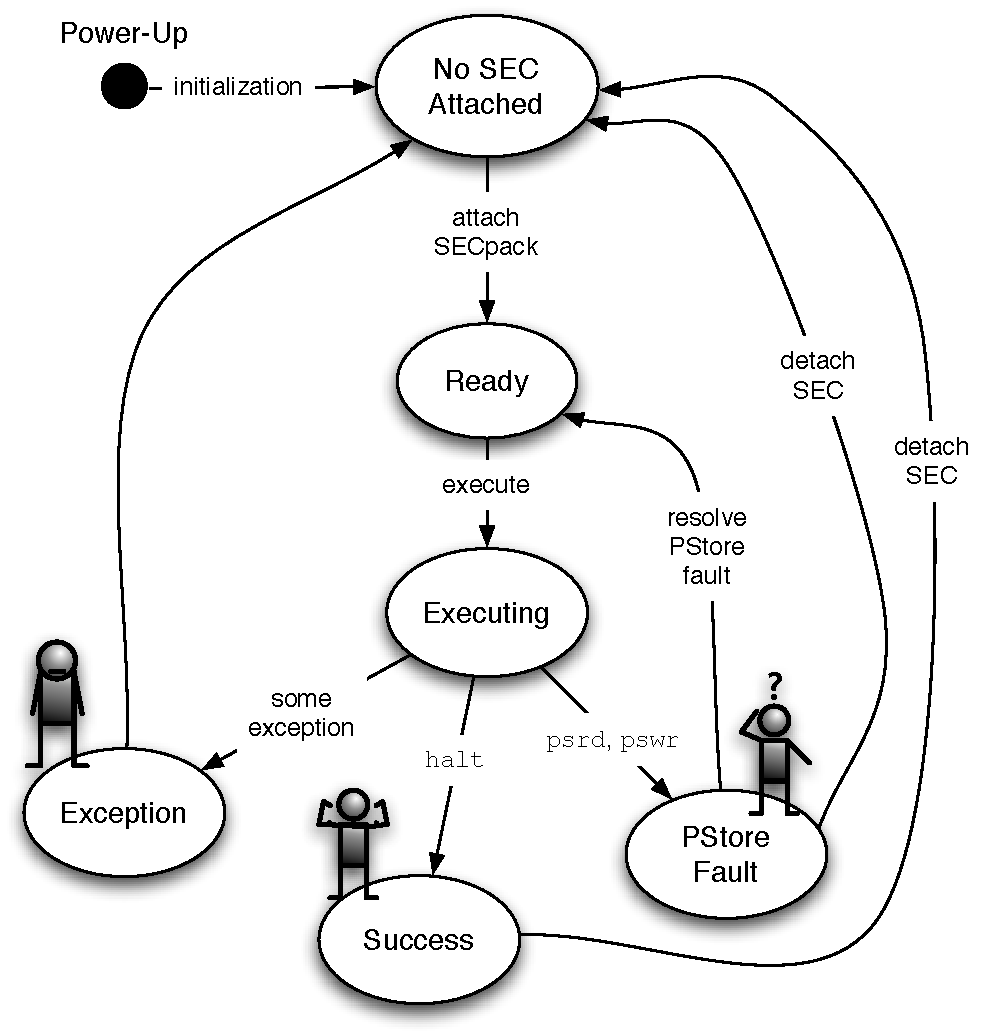
\includegraphics{omnifigs/execution_states}
	}
	\caption{State Machine for the TEM's Execution Engine}
	\label{fig:exec_states}
\end{figure}


\subsection{Development Support}\label{impl:fw_dev_support}
The prototype TEM implementation contains supplemental features to help
debugging SEClosures. These features are usually associated with ``developer
versions'' of chips.

When an exception occurs, the state of the VM interpreter is saved, using the
same code path as for persistent store faults. Detaching an exception-causing
SEClosure from the execution engine returns the interpreter state to the driver
software. The prototype driver implementation uses the information to show the
user the line of code containing the VM instruction that caused the exception.
Section \ref{impl:driver_dev_support} describes the driver side of the
mechanism and shows a processed SEClosure execution exception.

The prototype TEM is also capable of producing a list of the buffers
allocated by the memory managers, as well as a list of the keys in the
persistent store. This information is also processed by the prototype driver,
producing the snapshot shown in section \ref{impl:driver_dev_support}.

In order to ensure that the development features do not interfere with a
closure's confidentiality requirements, the SECpack header contains a flag that
indicates if development support features are allowed to be used with that
SECpack.

\subsection{Performance Considerations}
The table below shows the results of various tests that were run on two
JavaCard models. The times are expressed in seconds, and are averaged over
multiple repetitions of each operation. The number of repetitions was chosen
such that the results of running an experiment 3 times were within 1\% of the
mean.

\begin{center}
\begin{tabular}{|l|r|r|}
\hline
\textbf{Operations} & \textbf{NXP 41/72k} & \textbf{Philips 21 18k} \\
\hline
Process APDU & 0.0061 s & 0.029 s \\
\hline
Create and release 512-byte buffer & 0.084 s & 0.98 s \\
\hline
Decrypt with PrivEK & 0.76 s & 1.60 s \\
\hline
Execute 1-op SECpack & 0.16 s & 0.50 s \\
\hline
Execute 1020-ops SECpack & 0.82 s & 1.99 s \\
\hline
Execute 1-op bound SECpack & 0.89 s & 1.92 s \\
\hline
Execute 1020-ops bound SECpack & 1.53 s & 3.07 s \\
\hline
\end{tabular}
\end{center}

The SECpack execution performance is nothing to write home about, because
implementing the TEM's execution engine in JavaCard translates to writing a
virtual machine on top of another virtual machine. Usually, the speed difference
between native and interpreted code is on the order of 20X, so it is fair to
assume that a native implementation of the TEM's VM interpreter will be able
to process SECpack instructions an order of magnitude faster.

Despite the overhead introduced by the Java VM, the TEM was able to execute
SEClosures fast enough to make the demos described in section \ref{impl:demos}
work. This is a promising result which reinforces the point that most of a
SEClosure's execution time is spent on cryptographic operations that are
implemented in hardware and do not incur any VM-related overhead.

\section{Smartcard Access Extension to Ruby}\label{impl:rubygem}
I have implemented a Ruby extension that provides access to PC/SC smart card
readers, and was tested to work on Windows XP and Vista, Mac OS X Tiger and
Leopard, as well as Ubuntu Linux versions 7.10 and 8.04. The extension is
packaged using RubyGems \cite{berube2007forge}, the de-facto Ruby software
packaging standard. The extension has been placed under the MIT license, and
released on the Rubyforge site \cite{berube2007forge}, which makes the gem
readily avaible on any RubyGems-enabled Ruby interpreter, via the command
\texttt{gem install smartcard} .

\subsubsection{Motivation}
The first TEM driver was implemented in Java. The choice seemed natural, as my
JavaCard IDE came with Java libraries that interacted with the cards. However,
Java's lack of advanced language features makes it inadequate for assembling
SECpacks. Writing a proper assembler would have required a lot of effort, and
assembling SECpacks by hand became unattractive once I started using complex
SECpacks. This impacted research negatively, as I had less enthusiasm to
experiment.

The opportunity for tossing away the Java code presented itself when a
requirement was introduced that the TEM's demo software must be able to run on
both Mac OS X, and Linux. Java's libraries for smart card access were not well
developed for Mac OS X, so at that point it became reasonable to invest effort
into writing a Ruby extension, as opposed to a Java JNI library.

\subsubsection{Features}
When running under Windows, the gem uses the native PC/SC access library,
\texttt{winscard}. Under Linux or Mac OS X, the gem uses the \texttt{pcsclite}
library, which is a free port of a subset of \texttt{winscard}. All the
functions in \texttt{pcsclite} are exposed using an object-oriented interface,
and the gem code works around the peculiarities\footnote{bugs} in the PC/SC
implementations it targets.

\section{Driver Software for the TEM Host}\label{impl:driver}
The prototype implementation of the TEM's driver is not at all what one would
expect to find in a driver. The low-level details of communicating with the
TEM smart card are handled by the \textsc{smartcard} Ruby extension described
in section \ref{impl:rubygem}. Ruby makes encoding and decoding APDUs trivial,
as demonstrated by listing \ref{impl:driver_alloc_buffer}, which contains the
code for allocating a buffer on the TEM. This left time and energy for higher
level features that are rarely present in production drivers, let alone
research prototypes.

\lstinputlisting[float=bph, language=Ruby, caption=TEM Buffer Allocation
Implementation in the Ruby Driver,
label=impl:driver_alloc_buffer]{code/drv_alloc_buffer.rb}

\subsection{Domain Specific Languages}
Ruby is a highly dynamic language, and it is very suited for producing DSLs
(domain-specific languages), as demonstrated in \cite{cuadrado2007bds} and
\cite{cunningham2007rmr}. DSLs are part of the ``magic'' that is responsible
for the huge success of the Ruby on Rails \cite{thomas2006awd} framework. The
TEM driver uses two DSLs directly. A small language describes the primitive
data types on a TEM, and a second-order DSL\footnote{(a DSL that generates
another DSL)} expresses all the necessary information for assembling SEClosures.

The primitive data types DSL takes types one-line type definitions and
produces functions necessary for encoding and decoding numbers corresponding to
these data types. For instance, the definition for \texttt{byte} at the
beginning of listing \ref{impl:driver_types_dsl} yields the methods
\texttt{read\_tem\_byte}, \texttt{to\_tem\_byte}, and
\texttt{tem\_byte\_length}.

\lstinputlisting[float, language=Ruby, caption=TEM Primitive Data Types
Expressed using the DSL, label=impl:driver_types_dsl]{code/drv_types_dsl.rb}

The DSL describing the instruction set of the TEM is a second-order DSL. The
instruction set DSL, illustrated in listing \ref{impl:driver_instructions_dsl},
constitutes the backbone of the TEM assembler. An instruction definition in the
DSL contains user-friendly names for the instruction and its parameters, as
well as precise instructions on how to encode the instruction for the TEM's VM.

\lstinputlisting[float, language=Ruby, caption=Memory Block Instructions
Expressed using the DSL,
label=impl:driver_instructions_dsl]{code/drv_instructions_dsl.rb}

The Ruby driver features a state of the art SECpack assembler that supports
commens, multiple instructions per line, named parameters, named labels,
human-readable immediates, macros written in Ruby, and line-level debugging
information (exploited for the advanced developer support described  in section
\ref{impl:driver_dev_support}). Relating to the bank account example introduced
in section \ref{concepts:closures}, listing \ref{impl:driver_balance_secpack}
shows a possibile implementation of the \texttt{balance} SEClosure. The power of
the assembly language is illustrated well by the SECpack source in listing
\ref{impl:driver_keygen_secpack}. Most features were obtained at very little
cost, by using a DSL to represent the assembly language. This DSL is generated
from the instruction set DSL described above.

\lstinputlisting[float=hbt, language=Ruby,
caption=Assembly code for \texttt{balance} in the bank account example,
label=impl:driver_balance_secpack]{code/drv_balance_secpack.rb}

\lstinputlisting[float=hbt, language=Ruby, caption=Assembly Code for
Key-Generating SECpack, label=impl:driver_keygen_secpack]{code/drv_keygen_secpack.rb}

The set of DSLs presented here made experimenting fun again. Once the code for
interpreting the DSLs was solid, and the initial definitions were created, it
became really easy to change the definitions to experiment variations in
encoding data types or instructions. Because the DSLs are so easy to maintain,
they have become the authoritative specifications for the TEM's encoding
mechanisms.

\subsection{Developer Support}\label{impl:driver_dev_support}
The powerful assembly language described above plays a major role in making it
easy to develop SEClosures for the TEM. The other two big features are a full
suite of unit tests, and meaningful translations for SEClosure execution errors.

The TEM driver contains a full\footnote{\texttt{rcov} indicates a line coverage
of 95\% or above on each Ruby source file.} suite of unit tests, covering both
driver and firmware code. The unit tests have proven to be a very good
investment, as they have automated the following tasks:
\begin{itemize}
  \item validating the Ruby driver implementation,
  \item validating any TEM firmware implementation, 
  \item assessing the suitability of a JavaCard model as a TEM, and
  \item assessing the compatibility of a smart card reader with the TEM driver
  stack.
\end{itemize}

When any of the layers above exhibits a bug, a failing unit test provides a good
starting point for investigation. However, if the failure is a SEClosure execution exception, the Ruby driver goes one step further, by retrieving the TEM's execution engine status (using the features in section
\ref{impl:fw_dev_support}), and combining it with line-level debugging
information. The result is the ability to pinpoint the exact SECpack
instruction that caused the failure. Listing \ref{impl:driver_exception} shows
the data obtained from a typical SEClosure execution exception. Quick inspection
reveals that the exception occured during the \texttt{outw} instruction, and the
instruction was assembled in file \texttt{test\_exceptions.rb} at line 32. The
information includes a snapshot of the execution environment at the time of the
exception.

\lstinputlisting[float, language=Ruby, caption=Debugging Information for a SEClosure Execution Exception, label=impl:driver_exception]{code/drv_exception.txt}

This level of support is hard to find in research prototypes. It is present in
the TEM's driver because Ruby's dynamic features drove the cost of implementing
the features below the time that they saved.
\section{Demonstration Software}\label{impl:demos}
The TEM stack described in sections \ref{impl:firmware} - \ref{impl:driver} was
used to build the following small demonstrations:
\begin{itemize}
  \item An OpenSSL \cite{engelschall2001oos} engine using SECpacks as keys.
  When the engine is asked to generate an asymmetric key, it generates a
  2048-bit RSA key, and embeds the private key into SEClosures that encrypt,
  decrypt, and sign their arguments. The OpenSSL engine then performs all the 
  private key operations using SEClosures.
  \item A personal DRM system that uses SECpacks to store the authorization
  information for a media file. The file is broken into fixed-size blocks
  encrypted with indivual keys. The SEClosure that grants access to a file has a 
  master key used to generate the decryption keys. The SEClosure also contains
  code that expresses the permissions that the owner has (e.g., play this song at
  most 5 times, or distribute it to at most 3 friends.) The TEM provides a secure
  environment for the execution of the DRM policy code (what permissions a user
  does), and is intended to be used in conjunction with, not as a replacement
  for, secure audio playback hardware.
  \item A distributed file system that uses the TEM to insure the freshness of
  the file system's extents, which are stored on untrusted media. The servers
  use SEClosures to implement a trusted monotonic counter.
\end{itemize}

The demonstrations above show that the implementation described in this chapter
is functional and delivers acceptable performance. The chosen scenarios do not
showcase the full potential of the TEM.


\appendix
\chapter{Acronyms}

\begin{tabular}{llr}
\textbf{Term} & \textbf{Meaning} & \textbf{Defined In} \\
DSL & Domain-Specific Language & \ref{impl:driver} \\
ECert & Endorsement Certificate & \ref{concepts:trust_chain} \\
EK & Endorsement Key & \ref{concepts:trust_chain} \\
IP & Instruction Pointer & \ref{arch:vm} \\
PrivCA & Private Certificate Authority Key & \ref{concepts:trust_chain} \\
PrivEK & Private Endorsement Key & \ref{concepts:trust_chain} \\
PubCA & Public Certificate Authority Key & \ref{concepts:trust_chain} \\
PubEK & Public Endorsement Key & \ref{concepts:trust_chain} \\
SEClosure & Security-Enhanced Closure & \ref{concepts:secure_closures} \\
SECpack & A SEC that is compiled and encoded for the TEM &
\ref{concepts:secure_closures} \\
SP & Stack Pointer & \ref{arch:vm} \\
TEM & Trusted Execution Module & Abstract \\
TPM & Trusted Platform Module & \ref{intro:tpm} \\
VM & Virtual Machine & \ref{arch:vm} \\
\end{tabular}

%\chapter{Tables}

\begin{table}
\caption{Armadillos}
\label{arm:table}
\begin{center}
\begin{tabular}{||l|l||}\hline
Armadillos & are \\\hline
our	   & friends \\\hline
\end{tabular}
\end{center}
\end{table}

\clearpage
\newpage


%% This defines the bibliography file (main.bib) and the bibliography style.
%% If you want to create a bibliography file by hand, change the contents of
%% this file to a `thebibliography' environment.  For more information 
%% see section 4.3 of the LaTeX manual.
\begin{singlespace}
\bibliography{main}
\bibliographystyle{plainurl}
\end{singlespace}

\end{document}
